\documentclass{article}
\usepackage[margin=3cm]{geometry}
\usepackage{amsmath,amssymb,mathtools}
\usepackage[noend]{algpseudocode}
\usepackage{capt-of}
\usepackage{array}
\usepackage{tikz}
\usetikzlibrary{arrows.meta,positioning,fit,calc,decorations.pathreplacing}
\usepackage{hyperref}
\hypersetup{hidelinks}
\makeatletter
\providecommand*{\theHALG@line}{}
\renewcommand*{\theHALG@line}{\thefigure.\arabic{ALG@line}}
\makeatother
\pagestyle{plain}

% Objects and fields.
\newcommand{\genesis}{B_{\mathrm{gen}}}
\newcommand{\slot}{\operatorname{slot}}
\newcommand{\parent}{\mathsf{parent}}
\newcommand{\proposer}{\mathsf{proposer}}
\newcommand{\valindex}{\mathsf{val\_index}}
\newcommand{\round}{\mathsf{round}}
\newcommand{\rootf}{\mathsf{root}}
\newcommand{\committee}{\mathcal K}
\newcommand{\acp}{\mathsf{ac\_payload}}

% Chain state.
\newcommand{\targetParticipation}{\mathsf{target\_participation}}
\newcommand{\progressBit}{\mathsf{progress}}
\newcommand{\Qtarget}{Q_{\mathrm{target}}}
\newcommand{\Qprog}{Q_{\mathrm{prog}}}
\newcommand{\pendingFinality}{\mathsf{pending\_finality}}
\newcommand{\finalityParticipation}{\mathsf{finality\_participation}}
\newcommand{\Qfin}{Q_{\mathrm{fin}}}

% Store, frame and fork choice.
\newcommand{\T}{\mathcal T}
\newcommand{\hmax}{h_{\max}}
\newcommand{\AC}{\mathcal A}
\newcommand{\Fr}{\Phi}
\newcommand{\tree}{\mathsf{tree}}
\newcommand{\fcroot}{\mathsf{fc\_root}}
\newcommand{\allowed}{\mathsf{viable\_heads}}
\newcommand{\filtered}{\fname{viable\_tree}}
\newcommand{\gfPool}{\mathsf{gf\_votes}}
\newcommand{\attestations}{\mathsf{attestations}}
\newcommand{\fname}[1]{\text{\textsc{#1}}}
\newcommand{\latestConfirmed}{\mathsf{latest\_confirmed}}
\newcommand{\timestamp}{\mathsf{timestamp}}
\newcommand{\resolutionTime}{\mathsf{resolution\_time}}

% AC state.
\newcommand{\savedConfirmation}{\mathsf{saved\_confirmation}}
\newcommand{\locks}{\mathsf{locks}}
\newcommand{\restartTime}{\mathsf{restart\_time}}
\newcommand{\fgReported}{\mathsf{fg\_reported}}
\newcommand{\votedSlot}{\mathsf{voted\_slot}}

\title{Goldilocks}
\author{}
\date{}

\begin{document}
\maketitle

Goldilocks is an available chain, Goldfish with locks, composed with a
finality gadget.  The composition has three parts.  The \emph{finality gadget} (FG) keeps the
block tree, the chain state of every block, the finality caches and the
attestation pool; it decides which blocks are accepted, and it has the
validator client.  The \emph{available chain} (AC) is a protocol with its
own state, its own wire messages and its own part of a block; of the FG it
reads the FG frame and nothing else.  The \emph{node} keeps the clock and
the two states, runs the handlers and the duties, and calls the other two
parts.  Section~\ref{sec:composition} gives the node and the two
interfaces; it does not depend on the choice of the AC.
Section~\ref{sec:fg} gives the FG.  Section~\ref{sec:sa} gives the AC of
Goldilocks.  Figure~\ref{fig:system} shows the parts and the data
that pass between them.

\begin{center}
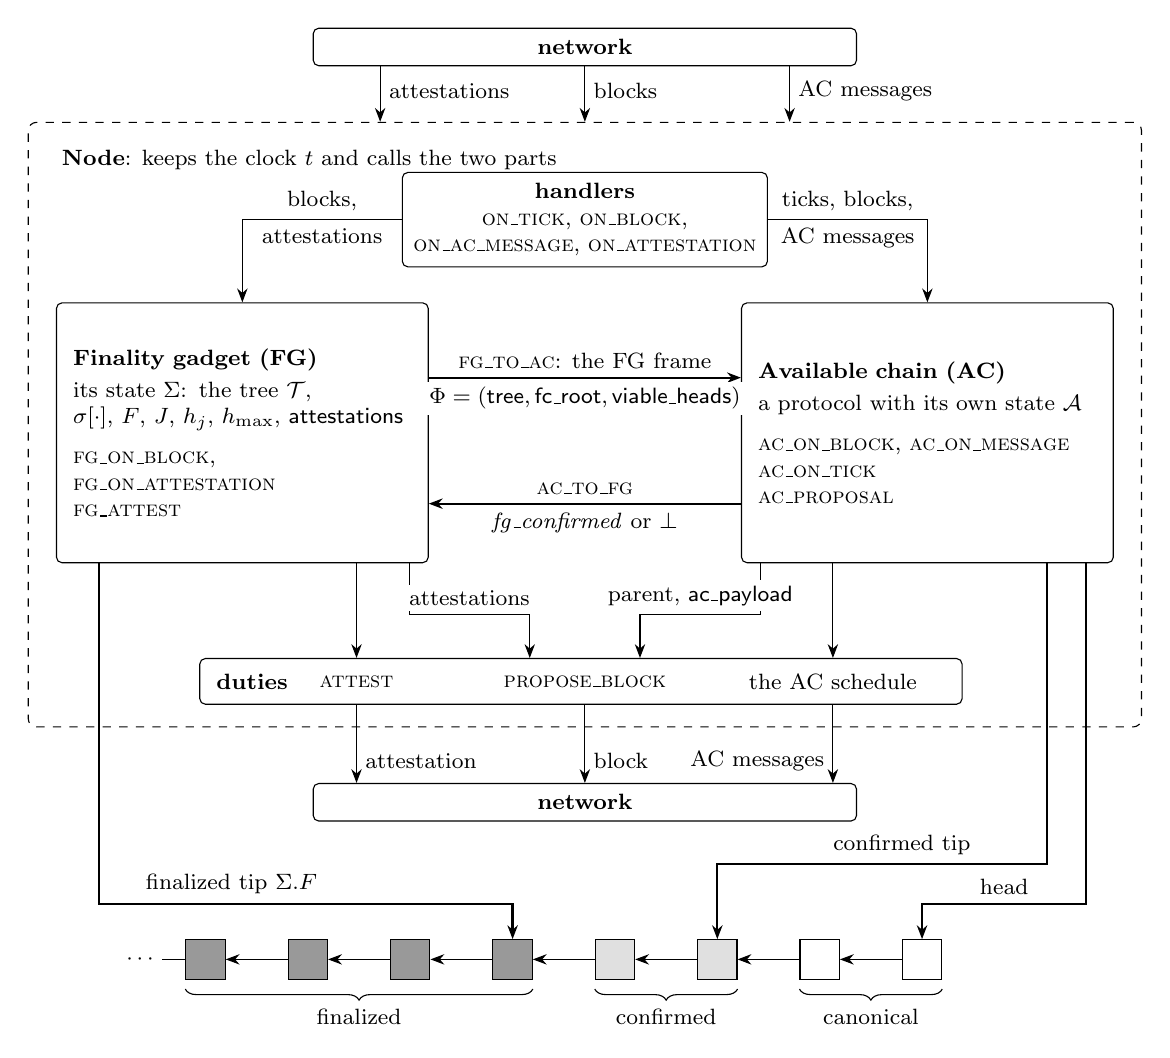
\begin{tikzpicture}[
  font=\footnotesize,
  >={Stealth[length=5pt]},
  part/.style={draw, rounded corners=2pt, align=left, inner sep=6pt,
    text width=4.3cm, minimum height=3.3cm, anchor=north west},
  small/.style={draw, rounded corners=2pt, align=center, inner sep=4pt},
  io/.style={align=center, inner sep=2pt},
  lab/.style={align=center, inner sep=2pt, fill=white},
]
% The two parts.
\node[part] (fg) at (0,0) {%
  \textbf{Finality gadget (FG)}\\[2pt]
  its state~$\Sigma$: the tree~$\T$,\\
  $\sigma[\cdot]$,\ $F$,\ $J$,\ $h_j$,\ $\hmax$, $\attestations$\\[5pt]
  $\fname{fg\_on\_block}$,\ $\fname{fg\_on\_attestation}$\\
  $\fname{fg\_attest}$};
\node[part] (ac) at (8.7,0) {%
  \textbf{Available chain (AC)}\\[2pt]
  a protocol with its own state~$\AC$\\[5pt]
  $\fname{ac\_on\_block}$,\ $\fname{ac\_on\_message}$\\
  $\fname{ac\_on\_tick}$\\
  $\fname{ac\_proposal}$};
% The interface.
\draw[->, thick] ($(fg.east)+(0,0.7)$) -- ($(ac.west)+(0,0.7)$)
  node[lab, midway, above=1pt] {$\fname{fg\_to\_ac}$: the FG frame}
  node[lab, midway, below=1pt] {$\Fr=(\tree,\fcroot,\allowed)$};
\draw[->, thick] ($(ac.west)+(0,-0.9)$) -- ($(fg.east)+(0,-0.9)$)
  node[lab, midway, above=1pt] {$\fname{ac\_to\_fg}$}
  node[lab, midway, below=1pt] {$\mathit{fg\_confirmed}$ or $\bot$};
% Handlers.
\node[small] (hand)
  at ($(fg.north east)!0.5!(ac.north west)+(0,1.05)$)
  {\textbf{handlers}\\
   $\fname{on\_tick}$,\ $\fname{on\_block}$,\\
   $\fname{on\_ac\_message}$,\ $\fname{on\_attestation}$};
\draw[->] (hand.west) -| (fg.north)
  node[lab, pos=0.25, above=1pt] {blocks,}
  node[lab, pos=0.25, below=1pt] {attestations};
\draw[->] (hand.east) -| (ac.north)
  node[lab, pos=0.25, above=1pt] {ticks, blocks,}
  node[lab, pos=0.25, below=1pt] {AC messages};
% Duties: one box, narrower than the two parts.
\node[io] (att) at ($(fg.south)+(1.45,-1.5)$) {$\fname{attest}$};
\node[io] (prop) at ($(fg.south east)!0.5!(ac.south west)+(0,-1.5)$)
  {$\fname{propose\_block}$};
\node[io] (vote) at ($(ac.south)+(-1.2,-1.5)$) {the AC schedule};
\node[draw, rounded corners=2pt, inner sep=4pt,
  fit={($(fg.south |- att.north)+(-0.4,0)$)
       ($(ac.south |- att.south)+(0.3,0)$)}] (duties) {};
\node[anchor=west, inner sep=2pt] at ($(duties.west)+(4pt,0)$)
  {\textbf{duties}};
\draw[->] (att.north |- fg.south) -- (att.north |- duties.north);
\draw[->] ($(fg.south east)+(-0.25,0)$) -- ++(0,-0.65)
  -| ($(prop.north |- duties.north)+(-0.7,0)$)
  node[lab, pos=0.25, above=1pt] {attestations};
\draw[->] ($(ac.south west)+(0.25,0)$) -- ++(0,-0.65)
  -| ($(prop.north |- duties.north)+(0.7,0)$)
  node[lab, pos=0.25, above=1pt] {parent, $\acp$};
\draw[->] (vote.north |- ac.south) -- (vote.north |- duties.north);
% The node.
\node[anchor=south west, inner sep=2pt] (title)
  at ($(fg.north west)+(0,1.6)$)
  {\textbf{Node}: keeps the clock~$t$ and calls the two parts};
\node[draw, dashed, rounded corners=3pt, inner xsep=10pt, inner ysep=8pt,
  fit=(fg)(ac)(hand)(title)(duties)] (node) {};
% The network, above and below.
\node[small, minimum width=6.9cm] (netin)
  at ($(hand.north |- node.north)+(0,0.95)$) {\textbf{network}};
\foreach \dx/\txt in {-2.6/attestations, 0/blocks, 2.6/AC messages}
  \draw[->] ($(netin.south)+(\dx,0)$) -- ($(netin.south |- node.north)+(\dx,0)$)
    node[io, pos=0.45, right=1pt] {\txt};
\node[small, minimum width=6.9cm] (netout)
  at ($(prop.south |- node.south)+(0,-0.95)$) {\textbf{network}};
\draw[->] (att.south |- duties.south) -- (att.south |- netout.north)
  node[io, pos=0.72, right=1pt] {attestation};
\draw[->] (prop.south |- duties.south) -- (prop.south |- netout.north)
  node[io, pos=0.72, right=1pt] {block};
\draw[->] (vote.south |- duties.south) -- (vote.south |- netout.north)
  node[io, pos=0.72, left=1pt] {AC messages};
% The chain, with the outputs.
\coordinate (cy) at ($(fg.west |- netout.south)+(0,-1.75)$);
\foreach \i in {0,...,7}
  \node[draw, minimum size=0.5cm, inner sep=0pt] (b\i)
    at ($(cy)+(1.9+1.3*\i,0)$) {};
\foreach \i in {0,...,3}
  \node[draw, fill=black!40, minimum size=0.5cm, inner sep=0pt]
    at (b\i) {};
\foreach \i in {4,5}
  \node[draw, fill=black!12, minimum size=0.5cm, inner sep=0pt]
    at (b\i) {};
\node[io] at ($(b0.west)+(-0.55,0)$) {$\cdots$};
\draw (b0.west) -- ++(-0.3,0);
\foreach \i/\j in {0/1,1/2,2/3,3/4,4/5,5/6,6/7}
  \draw[<-] (b\i.east) -- (b\j.west);
\draw[decorate, decoration={brace, mirror, amplitude=4pt}]
  ($(b0.south west)+(0,-0.12)$) -- ($(b3.south east)+(0,-0.12)$)
  node[io, midway, below=5pt] {finalized};
\draw[decorate, decoration={brace, mirror, amplitude=4pt}]
  ($(b4.south west)+(0,-0.12)$) -- ($(b5.south east)+(0,-0.12)$)
  node[io, midway, below=5pt] {confirmed};
\draw[decorate, decoration={brace, mirror, amplitude=4pt}]
  ($(b6.south west)+(0,-0.12)$) -- ($(b7.south east)+(0,-0.12)$)
  node[io, midway, below=5pt] {canonical};
\draw[->, thick] ($(fg.south west)+(0.55,0)$) |- ($(b3.north)+(0,0.45)$)
  node[io, pos=0.66, above=1pt] {finalized tip $\Sigma.F$}
  -- (b3.north);
\draw[->, thick] ($(ac.south east)+(-0.85,0)$) |- ($(b5.north)+(0,0.95)$)
  node[io, pos=0.72, above=1pt] {confirmed tip}
  -- (b5.north);
\draw[->, thick] ($(ac.south east)+(-0.35,0)$) |- ($(b7.north)+(0,0.45)$)
  node[io, pos=0.75, above=1pt] {head}
  -- (b7.north);
\end{tikzpicture}
\captionof{figure}{The three parts.  The handlers feed each part from
the network, and the duties send to it.  The outputs point into one
chain: the finalized tip from the FG, and the confirmed tip and the head
from the AC.  $\fname{ac\_to\_fg}$ returns only $\mathit{fg\_confirmed}$
(or~$\bot$), which the node passes to the FG; the FG does not read the
head.}
\label{fig:system}
\end{center}

\paragraph{The name.}
Goldilocks is Goldfish with locks.  The name also says what the locks are
for.  Goldfish counts only the votes of one slot: it remembers too little
to keep a confirmed block when votes are missing.  A fork choice that
counts the latest vote of every validator, with no limit of age,
remembers too much.  A lock holds a confirmed block for about $k$~slots and
then expires: a memory that is neither too short nor too long.  The name
also fits the three tips of the chain.  The head is the newest, and it can
still change.  The finalized tip cannot change, but it comes late.  The
confirmed tip, the output of the available chain, is between the two: it
comes soon, and the locks protect it.

\section{Composition}\label{sec:composition}

\subsection{Model}\label{sec:model}

A fixed set~$V$ of $n\geq1$ validators is given.  Every validator has
weight~$1$: for $S\subseteq V$, $w(S)=|S|$, and the quorum threshold is
$q=\lceil 2n/3\rceil$.  $\Delta$ is the delivery parameter of blocks and
AC messages, and $\Delta_F\geq\Delta$ is the delivery parameter of
attestations.  A bound is strict: the receiver processes the object at
a time strictly less than the deadline of the bound.  When the deadline is
a public time, the receiver thus processes the object before the tick at
that time.  Time is continuous, and the clock~$t$ of a node is the
current time.  The public times are the multiples of~$\Delta$.  A node
runs one tick at each public time.  A tick starts from the state as it
was before its public time, and each step of the tick reads the state
after the earlier steps of that tick.

A node is awake or asleep.  An asleep node receives nothing and runs no
tick, so it has no duty and no output.  An object that is sent while its
receiver sleeps, or that is not yet delivered when its receiver goes to
sleep, is delivered after the next wake: a delivery bound counts from the
later of the send time and that wake.  The node stamps an object with its
time of receipt.  A node that wakes restarts (Section~\ref{sec:store})
before it runs a tick or processes an object at that time; a crash is a
sleep.

The delivery bounds hold for every awake honest node.  An honest node
forwards an object when it accepts it: a block when the FG accepts it, an
AC message when the AC admits it, and an attestation when it passes the
checks.  This includes the objects that a block carries: a vote that the AC
admits from the payload of an accepted block, and an attestation of an
accepted block that enters the pool, are forwarded as wire objects of their
own, whether or not another node accepts the block.  So a delivery bound also counts from the time at which an honest
node first accepts the object; a receipt that is refused is not forwarded.  A node that runs
while its delivery is under the control of the adversary is faulty.

Slot~$s$ starts at the public time~$t_s$, with $t_0=0$ and
$t_s<t_{s+1}$, and has an assigned proposer.  The slot of a time~$t$, written $\slot(t)$, is
the greatest~$s$ with $t_s\leq t$.  Round~$r$ has the slots
$rR,\ldots,rR+R-1$, and $\round(s)=\lfloor s/R\rfloor$.  Its opening time
is $T_r=t_{rR}$.  Rounds are the heartbeat of the network for the
aggregation of attestations; no rule of the shared node reads them, and an
AC can use them.  The AC fixes the slot times and a lower bound on~$R$.

The local validator index is~$\valindex$.

\subsection{Blocks}\label{sec:blocks}

Every block~$B$ has a root~$B.\rootf$, slot~$B.\slot$, parent~$B.\parent$,
and proposer index~$B.\proposer$.  It has an AC payload~$B.\acp$ and a list
$B.\mathsf{attestations}$ of attestations (the FG payload).  The
order of each list and its repeated entries are part of the block.  The
block names its parent by root; the FG state must hold that parent in full,
with the same content, not only a block with the same root.  $B.\rootf$
is the fixed digest of
\[
 (B.\parent.\rootf,\ B.\slot,\ B.\mathsf{attestations},\ B.\acp).
\]
The AC fixes the encoding of its payload in this input.

The proposer signs a block with the slot key of $B.\proposer$.  A
validator signs an attestation with its fixed identity $\valindex\in V$.
A handler receives an object only when its signature is valid for its
signer and these checks pass: the signer of an attestation is in~$V$ and
its pairs have the forms of Section~\ref{sec:fg}; the slot key of
$B.\proposer$ signs a block~$B$; every attestation
that $B$ carries passes the same checks as on the wire;
$\Call{ac\_valid\_payload}{B}$ holds; an AC message passes the checks of
the AC; and $B.\rootf$ is the digest of the content of~$B$.  The check
drops an object that fails it, with no effect.

Processed blocks form a parent-closed tree rooted at~$\genesis$.  Write
$B\preceq C$ when $B=C$ or $B$ is an ancestor of~$C$, and write $B\prec C$
for strict ancestry.  Two blocks are compatible when one is an ancestor of
the other, and they conflict otherwise.  The depth of a block is the
number of parent edges from genesis.  ``Deepest'' means maximum depth;
ties use a fixed root order.

\subsection{State}\label{sec:store}

The node keeps the clock~$t$, the FG state~$\Sigma$ and the AC
state~$\AC$.  The FG state is
\[
 \Sigma=(\T,\sigma[\cdot],F,J,h_j,\hmax,\attestations).
\]
$\Sigma.\T$ is the tree of accepted blocks.  A block enters it only when
it extends~$\Sigma.F$, and no rule removes a block.
$\Sigma.\sigma[B]$ is the immutable chain state of an accepted
block.  $\Sigma.F$, $\Sigma.J$, $\Sigma.h_j$ and $\Sigma.\hmax$ are the
finality caches.  Section~\ref{sec:fg} defines the chain state and the
caches.  $\Sigma.\attestations$ holds
the processed attestations in full, one copy of each, in the order of
first acceptance, with no age limit and no limit per validator.  No rule
reads the time at which an attestation arrived; the pool serves inclusion
only.  Attestations reach the pool on the wire, through the node's own
$\Call{attest}{}$, and from the blocks that the FG accepts, after the
block's finality update.

Only the FG functions read and write~$\Sigma$, and only the AC functions
read and write~$\AC$.  The AC has no block store: the FG decides which
blocks are accepted, and the AC sees them through the FG frame.

The validator also keeps its anti-slashing record~$\Lambda$
(Section~\ref{sec:fg}).  The record belongs to the validator.  It is
durable: it persists through a restart.  A restart keeps~$\Lambda$,
$\Sigma$ and the clock, and it replaces~$\AC$ by
$\Call{ac\_restart}{\AC,\Fr,t}$, with $\Fr=\Call{fg\_to\_ac}{\Sigma}$
and $t$ the time of the restart.  The AC decides which part of its state
persists.

At initialization, $t=0$,
\[
 \Sigma.\T=\{\genesis\},\quad
 \Sigma.F=\Sigma.J=\genesis,\quad \Sigma.h_j=0,\quad \Sigma.\hmax=1,
\]
$\Sigma.\sigma[\genesis]$ is the initial chain state, the pool is empty,
and $\AC$ is the initial state of the AC.

\subsection{The FG frame}\label{sec:frame}

The FG frame is what the FG gives to the AC.  It is derived from the FG
state when used, and every call of one tick step reads the FG frame of the
same state:
\[
 \Fr=\Call{fg\_to\_ac}{\Sigma}=(\tree,\fcroot,\allowed).
\]
\begin{itemize}
\item $\Fr.\tree$ is the set of the accepted blocks that
  extend~$\Sigma.F$.  Write $\Fr.F$ for its root, the block~$\Sigma.F$.
\item $\Fr.\fcroot$ is a block of $\Fr.\tree$: the root of the fork
  choice.
\item $\Fr.\allowed$ is a set of blocks of $\Fr.\tree$ that
  extend~$\Fr.\fcroot$: the blocks on which a head walk may stop.
\end{itemize}
For a set $\mathit{tree}\subseteq\Fr.\tree$, the \emph{viable tree}
$\filtered(\Fr,\mathit{tree})$ is the set of the blocks of~$\mathit{tree}$
that extend~$\Fr.\fcroot$ and have a descendant in
$\mathit{tree}\cap\Fr.\allowed$.  It follows from the FG frame; it is not a
part of it.
$\Fr.F$ moves only to a descendant, also through a restart, because a
restart keeps~$\Sigma$.  So a block that leaves $\Fr.\tree$ does not
return.  Figure~\ref{alg:fg-store} computes the FG frame.

\subsection{The available chain}\label{sec:ac-interface}

An AC has a state~$\AC$, a set of wire messages, a block payload, and
these functions.  $t$ is the clock of the node.
\[
\begin{array}{l@{\qquad}l}
 \Call{ac\_valid\_payload}{B} & \text{stateless check of $B.\acp$},\\
 \Call{ac\_on\_message}{\AC,\Fr,t,m} & \text{an AC wire message arrives},\\
 \Call{ac\_on\_block}{\AC,\Fr,t,B} & \text{the FG accepted block $B$},\\
 \Call{ac\_on\_tick}{\AC,\Fr,t} & \text{the schedule of the AC; it can
   send AC messages},\\
 \Call{ac\_proposal}{\AC,\Fr,t} & \text{returns
   $(H,\mathit{ac\_payload})$: a parent and an AC payload, or $\bot$},\\
 \Call{ac\_to\_fg}{\AC,\Fr,t} & \text{returns
   $\mathit{fg\_confirmed}$, or $\bot$ when no block is new},\\
 \Call{ac\_confirmed}{\AC,\Fr,t} & \text{returns the confirmed tip},\\
 \Call{ac\_head}{\AC,\Fr,t} & \text{returns the head},\\
 \Call{ac\_restart}{\AC,\Fr,t} & \text{returns the AC state after a restart}.
\end{array}
\]
The two receipt handlers $\Call{ac\_on\_message}{}$ and
$\Call{ac\_on\_block}{}$ can also send AC messages, as
$\Call{ac\_on\_tick}{}$ can.  These functions do not take the FG state.  The AC holds a block in its state only as
a name: the content of a block and its ancestry come from $\Fr.\tree$, or
from the block that a call supplies.  The AC must satisfy these
requirements.
\begin{enumerate}
\item Every head of a duty (the parent of a proposal, the head of a vote)
  extends~$\Fr.\fcroot$.
  Such a head whose walk starts in $\filtered(\Fr,\mathit{tree})$ is in
  $\Fr.\allowed$.
\item A block $\mathit{fg\_confirmed}$ other than~$\bot$ is in
  $\filtered(\Fr,\Fr.\tree)$.
\item The output of $\Call{ac\_head}{}$ extends~$\Fr.\fcroot$, and the
  confirmed tip extends~$\Fr.F$ and is an ancestor of that output.
\item The parent of a proposal is a head of the AC at that time.
\end{enumerate}

The protocol exposes three tips: the finalized tip~$\Sigma.F$, the
confirmed tip $\Call{ac\_confirmed}{\AC,\Fr,t}$ and the head
$\Call{ac\_head}{\AC,\Fr,t}$, with $\Fr=\Call{fg\_to\_ac}{\Sigma}$.  They
lie on one chain: the finalized tip is an ancestor of the confirmed tip,
and the confirmed tip is an ancestor of the head.

\subsection{Node}\label{sec:node}

The node runs the tick of a public time before it processes any object
received at that time.  It stamps an object with the time at which it
processes it, so an object received at a public time~$\tau$ counts as
received after the tick at~$\tau$.  A tick runs the schedule of the AC,
then the proposal duty at~$t_s$,
then the FG update.  A node processes its own block, its own AC
message and its own attestation at once.

The node drops a block of a future slot.  The FG then accepts the block
only when its full parent is held, no held block has its root, it
extends~$\Sigma.F$, and the assertions of its state transition hold.  A
failed test or assertion refuses the block before any write, and the AC
does not see a refused block.
No handler then runs for an object that it carries, and a later delivery
can call the handler again.  The proposer takes the parent and the AC
payload from the AC; when the AC returns~$\bot$, it makes no proposal.  It includes every attestation of its pool that is
valid against the state of the parent and is not already on the parent's
chain, in the order of its pool.

\emph{The FG update.}  After each tick the node asks the AC for an FG
update.  The AC returns a block $\mathit{fg\_confirmed}$, or~$\bot$ when
it has no new block to vouch for.
$\mathit{fg\_confirmed}$ is the block up to which the AC vouches for its
chain, for the FG.  The node gives the FG each such block, the
\emph{source}, and the
client record decides whether an attestation follows: a target only as the
first vote at a height, and no entry twice (Section~\ref{sec:fg}).  The
height pair comes from the chain state of the source, and the finality
pair from the entry state of that chain state
(Section~\ref{sec:fg-client}).

The node functions take the input from outside the node: the time of a
tick, a received object, or the output of the AC for a duty.  They read
the clock~$t$ and pass $\Sigma$, $\AC$ and~$\Lambda$ to the two parts.

\captionof{figure}{Node: handlers and duties}\label{alg:node}
\nopagebreak
{\footnotesize
\begin{algorithmic}[1]
\Function{on\_tick}{$t$}
  \Comment{at each public time $t$}
  \State $s\gets\slot(t)$
  \State $\Fr\gets\Call{fg\_to\_ac}{\Sigma}$; \Call{ac\_on\_tick}{$\AC,\Fr,t$}
  \If{$s>0$ and $t=t_s$ and $\valindex$ is the slot-$s$ proposer}
    \State $P\gets\Call{ac\_proposal}{\AC,\Fr,t}$
    \Comment{$\bot$: the AC makes no proposal}
    \If{$P\neq\bot$} \State \Call{propose\_block}{$P$} \EndIf
  \EndIf
  \State $\Fr\gets\Call{fg\_to\_ac}{\Sigma}$;\quad
    $\mathit{fg\_confirmed}\gets\Call{ac\_to\_fg}{\AC,\Fr,t}$
  \Comment{$\bot$: no new block for the FG}
  \If{$\mathit{fg\_confirmed}\neq\bot$}
    \State \Call{attest}{$\mathit{fg\_confirmed}$}
    \Comment{the source}
  \EndIf
\EndFunction
\vspace{1pt}
\Function{on\_block}{$B$}
  \If{$B.\slot>\slot(t)$} \State \Return \EndIf
  \If{not $\Call{fg\_on\_block}{\Sigma,B}$} \State \Return
    \Comment{the FG accepts or refuses the block}
  \EndIf
  \State $\Fr\gets\Call{fg\_to\_ac}{\Sigma}$; \Call{ac\_on\_block}{$\AC,\Fr,t,B$}
    \Comment{the frame after the FG accepted $B$}
\EndFunction
\vspace{1pt}
\Function{on\_ac\_message}{$m$}
  \State $\Fr\gets\Call{fg\_to\_ac}{\Sigma}$; \Call{ac\_on\_message}{$\AC,\Fr,t,m$}
\EndFunction
\vspace{1pt}
\Function{on\_attestation}{$a$}
  \State \Call{fg\_on\_attestation}{$\Sigma,a$}
\EndFunction
\vspace{1pt}
\Function{propose\_block}{$(H,\mathit{ac\_payload})$}
  \Comment{runs at $t_s$}
  \State $B\gets$ a block with $B.\parent=H$, $B.\slot=\slot(t)$,
    $B.\proposer=\valindex$, $B.\acp=\mathit{ac\_payload}$
  \State $B.\mathsf{attestations}\gets
    \Call{proposal\_attestations}{\Sigma,H}$
  \State broadcast $B$; \Call{on\_block}{$B$}
\EndFunction
\vspace{1pt}
\Function{attest}{$\mathit{fg\_confirmed}$}
  \State $a\gets\Call{fg\_attest}{\Sigma,\Lambda,\mathit{fg\_confirmed}}$
  \If{$a=\bot$} \State \Return \EndIf
  \State broadcast $a$; \Call{on\_attestation}{$a$}
\EndFunction
\end{algorithmic}
}

\section{Finality gadget}\label{sec:fg}

\subsection{Attestations and chain state}\label{sec:fg-state}

An attestation is
\[
 a=(\valindex,h,T,\tau,h_f,T_f).
\]
Its height pair $(h,T,\tau)$ is a vote at height $h\geq1$ that names the
block $T\neq\bot$ that brought the chain into height~$h$ on the
chain of $\mathit{fg\_confirmed}$: a \emph{target vote} when $\tau=\mathsf{false}$, and a
\emph{timeout} when $\tau=\mathsf{true}$.  Its finality pair $(h_f,T_f)$ is
empty, $(\bot,\bot)$, or has $T_f\neq\bot$ and $h_f<h$.
An attestation names $T$ and~$T_f$ by root, as a block names its parent.  A
test that compares $T$ or~$T_f$ with a block, or a pair with a pair of
$\sigma.\pendingFinality$, compares roots.

The chain state of an accepted block is
\[
 \begin{gathered}
 \Sigma.\sigma[B]=\Call{state\_transition}{\Sigma.\sigma[B.\parent],B},\\
 \sigma=(L,s,h,T_h,\targetParticipation,\progressBit,\pendingFinality,\finalityParticipation[\cdot],J,h_j,F,h_F).
 \end{gathered}
\]
$\sigma.L$ is the latest block, $\sigma.s=\sigma.L.\slot$, $\sigma.h$ is
the current height, and $\sigma.T_h$ is the block that brought the chain
into height~$\sigma.h$.  The arrays $\sigma.\targetParticipation$ and
$\sigma.\progressBit$ hold one Boolean value per validator.  Their quorum
sets are derived when used:
$\Qtarget(\sigma)=\{i:\sigma.\targetParticipation[i]\}$ and
$\Qprog(\sigma)=\{i:\sigma.\progressBit[i]\}$.  The pair
$(\sigma.J,\sigma.h_j)$ is the latest justification on the chain, and
$(\sigma.F,\sigma.h_F)$ is its latest finalization.  $\sigma.\pendingFinality$ is a list of at most $K_W$ pairs $(j,T)$ in
increasing order of~$j$, with $\sigma.h_F<j\leq\sigma.h_j$: the chain
justified~$T$ at height~$j$ and has not finalized it.  For each pair
$(j,T)$ of the list, the array $\sigma.\finalityParticipation[j]$ holds
one Boolean value per validator: whether a finality pair of that
validator names $(j,T)$ on the chain.  Its quorum set is
$\Qfin(\sigma,j)=\{i:\sigma.\finalityParticipation[j][i]\}$.  The
\emph{entry state} of~$\sigma$ is $\Sigma.\sigma[\sigma.T_h]$, the state
of the block that brought the chain into height~$\sigma.h$; its height
is~$\sigma.h$.  A justification ends its height, so every state with the
entry $(\sigma.h,\sigma.T_h)$ has the pair $(\sigma.J,\sigma.h_j)$ of its
entry state.  The height~$\sigma.h$ has its \emph{previous height
justified} ($\Call{previous\_height\_justified}{\sigma}$) when
$\sigma.h_j>0$ and $\sigma.h_j=\sigma.h-1$: the chain entered it by
justifying its predecessor $(\sigma.h_j,\sigma.J)$.  $K_W=2$, and
$\delta_{\mathrm{t}}\geq0$ is the timeout delay in slots; the AC sets its
value (Section~\ref{sec:sa-schedule}).  Initially
\[
 \sigma.L=\sigma.T_h=\sigma.J=\sigma.F=\genesis,\quad
 \sigma.s=0,\quad \sigma.h=1,\quad \sigma.h_j=\sigma.h_F=0,
\]
every array entry is false, and $\sigma.\pendingFinality$ is empty.

Every attestation that a block includes must be valid against the
parent's state: the attestation names the current entry of that state, or
it is a vote below the height of that state whose finality pair is a
pending pair of that state.

\subsection{Finality caches and frame}\label{sec:fg-frame}

$\Sigma.F$ is the accepted finalization, $(\Sigma.J,\Sigma.h_j)$ is the
lex-greatest justification of the accepted states that
extends~$\Sigma.F$, and $\Sigma.\hmax$ is the greatest accepted state
height.  With the tree, the chain states and the pool, these caches are the FG
state.  The FG frame is derived from it when used.

\emph{Frontier contest.}  The FG state is \emph{contested} when
$\Sigma.\hmax=\Sigma.h_j+1$ and some accepted block that
extends~$\Sigma.F$, with state height~$\Sigma.\hmax$, does not
extend~$\Sigma.J$.  The test reads the whole tree and the finality caches,
never the tree of a voter.  In a contest, the fork-choice root is~$\Sigma.F$ and the head height floor
is~$\Sigma.\hmax$.  Otherwise the fork-choice root is~$\Sigma.J$ when
$\Sigma.\hmax=\Sigma.h_j+1$ and $\Sigma.F$ when not, and the head height floor
is $\Sigma.\hmax-1$.  The head height floor gives the viable heads: the blocks
at or above the fork-choice root whose state height is at least the head height floor.
A block is \emph{viable} when its state height is at least the head height
floor.  Finality acceptance uses the same test: $\Sigma.F$ advances only to
a block with a viable descendant.

\captionof{figure}{FG: handlers, finality caches and frame}\label{alg:fg-store}
\nopagebreak
{\footnotesize
\begin{algorithmic}[1]
\Function{fg\_on\_block}{$\Sigma,B$}
  \Comment{returns whether $B$ is accepted}
  \If{$B.\rootf$ is the root of a block of $\Sigma.\T$ or
      $B.\parent\notin\Sigma.\T$ or $\Sigma.F\not\preceq B$}
    \State \Return $\mathsf{false}$
  \EndIf
  \State $\Sigma.\sigma[B]\gets
    \Call{state\_transition}{\Sigma.\sigma[B.\parent],B}$
  \Comment{a failed assertion: no write, return $\mathsf{false}$}
  \State add $B$ to $\Sigma.\T$
  \State \Call{update\_finality}{$\Sigma,\Sigma.\sigma[B]$}
  \ForAll{$a\in B.\mathsf{attestations}$}
    \State \Call{fg\_on\_attestation}{$\Sigma,a$}
  \EndFor
  \State \Return $\mathsf{true}$
\EndFunction
\vspace{1pt}
\Function{fg\_on\_attestation}{$\Sigma,a$}
  \State add $a$ to $\Sigma.\attestations$
  \Comment{one copy of each attestation}
\EndFunction
\vspace{1pt}
\Function{fg\_attest}{$\Sigma,\Lambda,\mathit{fg\_confirmed}$}
  \State $(h_c,T_c)\gets(\Sigma.\sigma[\mathit{fg\_confirmed}].h,
    \Sigma.\sigma[\mathit{fg\_confirmed}].T_h)$
  \State $\sigma_e\gets\Sigma.\sigma[T_c]$
  \Comment{the entry state: $\sigma_e.h=h_c$, $\sigma_e.T_h=T_c$}
  \State \Return $\Call{create\_attestation}{\Lambda,h_c,T_c,\sigma_e}$
  \Comment{an attestation or $\bot$}
\EndFunction
\vspace{1pt}
\Function{update\_finality}{$\Sigma,\sigma$}
  \State $\Sigma.\hmax\gets\max(\Sigma.\hmax,\sigma.h)$
  \If{$\Sigma.F\preceq\sigma.J$ \textbf{and}
      $(\sigma.h_j,\sigma.J.\rootf)>(\Sigma.h_j,\Sigma.J.\rootf)$}
    \Comment{lex order}
    \State $(\Sigma.J,\Sigma.h_j)\gets(\sigma.J,\sigma.h_j)$
  \EndIf
  \If{$\Sigma.F\prec\sigma.F$ \textbf{and} $\sigma.F\preceq\Sigma.J$
      \textbf{and} $\Call{has\_viable\_descendant}{\Sigma,\sigma.F}$}
    \State $\Sigma.F\gets\sigma.F$
  \EndIf
\EndFunction
\vspace{1pt}
\Function{fg\_contest}{$\Sigma$}
  \If{$\Sigma.\hmax\neq\Sigma.h_j+1$} \State \Return $\mathsf{false}$ \EndIf
  \State $\mathit{hmax\_blocks}\gets\{B\in\Sigma.\T:\Sigma.F\preceq B,\
    \Sigma.\sigma[B].h=\Sigma.\hmax\}$
  \Comment{the whole tree, never the tree of a voter}
  \State \Return $\exists B\in\mathit{hmax\_blocks},\ \Sigma.J\not\preceq B$
\EndFunction
\vspace{1pt}
\Function{head\_height\_floor}{$\Sigma$}
  \If{$\Call{fg\_contest}{\Sigma}$} \State \Return $\Sigma.\hmax$ \EndIf
  \State \Return $\Sigma.\hmax-1$
\EndFunction
\vspace{1pt}
\Function{get\_fc\_root}{$\Sigma$}
  \If{$\Sigma.\hmax=\Sigma.h_j+1$ \textbf{and not} $\Call{fg\_contest}{\Sigma}$}
    \State \Return $\Sigma.J$
  \EndIf
  \State \Return $\Sigma.F$
\EndFunction
\vspace{1pt}
\Function{is\_viable}{$\Sigma,B$}
  \State \Return $\Sigma.\sigma[B].h\geq\Call{head\_height\_floor}{\Sigma}$
\EndFunction
\vspace{1pt}
\Function{has\_viable\_descendant}{$\Sigma,B$}
  \State \Return $\exists B'\in\Sigma.\T,\ B\preceq B',\
    \Call{is\_viable}{\Sigma,B'}$
\EndFunction
\vspace{1pt}
\Function{fg\_to\_ac}{$\Sigma$}
  \State $\mathit{tree}\gets\{B\in\Sigma.\T:\Sigma.F\preceq B\}$
  \State $\mathit{fc\_root}\gets\Call{get\_fc\_root}{\Sigma}$
  \State $\mathit{viable\_heads}\gets\{B\in\mathit{tree}:
    \mathit{fc\_root}\preceq B,\ \Call{is\_viable}{\Sigma,B}\}$
  \State \Return $(\mathit{tree},\mathit{fc\_root},\mathit{viable\_heads})$
\EndFunction
\vspace{1pt}
\Function{proposal\_attestations}{$\Sigma,H$}
  \State \Return the $a\in\Sigma.\attestations$ with
    $\Call{valid\_attestation}{\Sigma.\sigma[H],a}$ that are not on $H$'s chain,
  \Statex \hspace{2em}in the order of the pool
\EndFunction
\end{algorithmic}
}

\subsection{Validator client}\label{sec:fg-client}

The anti-slashing record is
\[
 \Lambda=(\mathsf{target}[\cdot],\mathsf{timeout}[\cdot],
 \mathsf{lock}[\cdot],\mathsf{sent}):
\]
for each height~$h$, the first target that the validator sent at~$h$,
the set of the blocks that its timeouts at~$h$ name, and the target of
its first finality pair at~$h$, initially $(\bot,\emptyset,\bot)$; and
the set of the contents (height pair and finality pair) of the
attestations that it sent, initially empty.
$\Call{record\_attestation}{}$ is its only writer.  The tests read only
whether $\mathsf{timeout}[h]$ is empty, one block, or more, so a client
can store it as $\bot$, a root, or a mark for two or more blocks.  A
record that stores a Boolean at $\mathsf{timeout}[h]$, as an earlier
version of this client did, gives no root: false reads as the empty set,
and true reads as two or more blocks, never as a set within~$\{T\}$.

The client sends an attestation only with a height pair.  It sends a
target at a height only as its first vote at that height, and it names
each entry at most once at a height.  After a finality pair $(h,T)$ it
sends no row at~$h$, timeout or target vote, that names another block.
It reads the finality pair from the entry state of its source, not from
the head.  At a height whose previous height is justified the
pair is the predecessor $(h_j,J)$ when the record allows it, also when a
later state has finalized it, and empty otherwise.  At another height it
is the newest pending pair of the entry state that the record allows, or
empty.  So the pair is below the height of the height pair.

\captionof{figure}{FG: validator client}\label{alg:attn-full}
\nopagebreak
{\footnotesize
\begin{algorithmic}[1]
\Function{finality\_pair}{$\Lambda,\sigma_e$}
  \Comment{$\sigma_e$: the entry state of the source}
  \If{$\Call{previous\_height\_justified}{\sigma_e}$}
    \Comment{the predecessor, even if a later state finalized it}
    \If{$\Call{permits}{\Lambda,\sigma_e.h_j,\sigma_e.J}$}
      \State \Return $(\sigma_e.h_j,\sigma_e.J)$
    \EndIf
    \State \Return $(\bot,\bot)$
  \EndIf
  \If{some $(j,T)\in\sigma_e.\pendingFinality$ has
      $\Call{permits}{\Lambda,j,T}$}
    \State \Return the one with the greatest~$j$
    \Comment{the newest permitted pair}
  \EndIf
  \State \Return $(\bot,\bot)$
\EndFunction
\vspace{1pt}
\Function{permits}{$\Lambda,j,T$}
  \Comment{the record allows the finality pair $(j,T)$}
  \State \Return $\Lambda.\mathsf{target}[j]\in\{\bot,T\}$ and
    $\Lambda.\mathsf{timeout}[j]\subseteq\{T\}$ and
    $\Lambda.\mathsf{lock}[j]\in\{\bot,T\}$
\EndFunction
\vspace{1pt}
\Function{height\_pair}{$\Lambda,h_c,T_c$}
  \If{$h_c=\bot$} \State \Return $(\bot,\bot,\bot)$ \EndIf
  \State $\mathit{lock}\gets\Lambda.\mathsf{lock}[h_c]$
  \If{$\mathit{lock}\notin\{\bot,T_c\}$}
    \State \Return $(\bot,\bot,\bot)$
    \Comment{locked elsewhere: wait out the height}
  \EndIf
  \If{$\Lambda.\mathsf{timeout}[h_c]\neq\emptyset$}
    \State \Return $(h_c,T_c,\mathsf{true})$
    \Comment{select a timeout for the current entry}
  \EndIf
  \If{$\Lambda.\mathsf{target}[h_c]\in\{\bot,T_c\}$}
    \State \Return $(h_c,T_c,\mathsf{false})$
    \Comment{vote for the target of that chain}
  \EndIf
  \State \Return $(h_c,T_c,\mathsf{true})$
  \Comment{otherwise time out at $h_c$}
\EndFunction
\vspace{1pt}
\Function{create\_attestation}{$\Lambda,h_c,T_c,\sigma_e$}
  \Comment{validator-client side: one chain state, no access to $\Sigma$}
  \State $(h_f,T_f)\gets\Call{finality\_pair}{\Lambda,\sigma_e}$
  \Comment{below $\sigma_e.h=h_c$}
  \State $(h,T,\tau)\gets\Call{height\_pair}{\Lambda,h_c,T_c}$
  \If{$h=\bot$} \State \Return $\bot$
    \Comment{no attestation without a height pair}
  \EndIf
  \If{some $b\in\Lambda.\mathsf{sent}$ has $b.h=h$ and ($\neg\tau$ or
      $b.T=T$)}
    \State \Return $\bot$
    \Comment{a target only as the first vote at $h$; no entry twice}
  \EndIf
  \State $a\gets(\valindex,h,T,\tau,h_f,T_f)$
  \State \Call{record\_attestation}{$\Lambda,a$}; \Return $a$
  \Comment{record, then send}
\EndFunction
\vspace{1pt}
\Function{record\_attestation}{$\Lambda,a$}
  \Comment{the only writer of $\Lambda$}
  \State add the content of $a$ to $\Lambda.\mathsf{sent}$
  \State $(h,T,\tau,h_f,T_f)\gets a$'s height and finality pairs
  \If{$T_f\neq\bot$} \State $\Lambda.\mathsf{lock}[h_f]\gets T_f$ \EndIf
  \If{$h\neq\bot$}
    \If{not $\tau$ and $\Lambda.\mathsf{target}[h]=\bot$}
      \State $\Lambda.\mathsf{target}[h]\gets T$
    \EndIf
    \If{$\tau$}
      \State $\Lambda.\mathsf{timeout}[h]\gets\Lambda.\mathsf{timeout}[h]\cup\{T\}$
    \EndIf
  \EndIf
\EndFunction
\end{algorithmic}
}

\captionof{figure}{FG: state transition}\label{alg:chain-full}
\nopagebreak
{\footnotesize
\begin{algorithmic}[1]
\Function{state\_transition}{$\sigma,B$}
  \State \textbf{assert} $B.\proposer=\operatorname{proposer}(B.\slot)$
  \State \textbf{assert} $B.\parent.\slot<B.\slot$
  \State \textbf{assert} every $a\in B.\mathsf{attestations}$ has
    $\Call{valid\_attestation}{\sigma,a}$
  \Comment{against the parent's state}
  \State $\sigma.s\gets B.\slot$
  \ForAll{$a\in B.\mathsf{attestations}$}
    \State $\sigma\gets\Call{process\_attestation}{\sigma,a}$
  \EndFor
  \State $\sigma.L\gets B$
  \State \Return $\Call{process\_height\_events}{\sigma}$
\EndFunction
\vspace{1pt}
\Function{valid\_attestation}{$\sigma,a$}
  \State $(h,T,\tau,h_f,T_f)\gets a$'s height and finality pairs
  \If{$(h,T)=(\sigma.h,\sigma.T_h)$}
    \State \Return $\mathsf{true}$
    \Comment{names the chain's own entry}
  \EndIf
  \State \Return $(h_f,T_f)\in\sigma.\pendingFinality$ and
    $h_f<h<\sigma.h$
  \Comment{an older vote with a useful finality pair}
\EndFunction
\vspace{1pt}
\Function{process\_attestation}{$\sigma,a$}
  \State $v\gets a.\valindex$;\quad
    $(h,T,\tau,h_f,T_f)\gets a$'s height and finality pairs
  \If{$(h_f,T_f)\in\sigma.\pendingFinality$}
    \State $\sigma.\finalityParticipation[h_f][v]\gets\mathsf{true}$
  \EndIf
  \If{$h=\sigma.h$ and $T=\sigma.T_h$}
    \Comment{names the chain's own entry}
    \State $\sigma.\progressBit[v]\gets\mathsf{true}$
    \If{not $\tau$}
      \State $\sigma.\targetParticipation[v]\gets\mathsf{true}$
    \EndIf
  \EndIf
  \State \Return $\sigma$
\EndFunction
\vspace{1pt}
\Function{process\_height\_events}{$\sigma$}
  \If{some $(j,T)\in\sigma.\pendingFinality$ has
      $w(\Qfin(\sigma,j))\geq q$}
    \State $(\sigma.F,\sigma.h_F)\gets(T,j)$ for the greatest such~$j$
  \EndIf
  \State remove from $\sigma.\pendingFinality$ every pair $(j,T)$ with
    $j\leq\sigma.h_F$
  \If{$w(\Qtarget(\sigma))\geq q$ \textbf{and}
      (not $\Call{previous\_height\_justified}{\sigma}$ or $\sigma.h_F=\sigma.h_j$)}
    \Comment{such a height waits for its predecessor}
    \State $(\sigma.J,\sigma.h_j)\gets(\sigma.T_h,\sigma.h)$
    \State append $(\sigma.h,\sigma.T_h)$ to $\sigma.\pendingFinality$;
      $\sigma.\finalityParticipation[\sigma.h]\gets\mathsf{false}^{V}$
    \State keep the newest $K_W$ pairs of $\sigma.\pendingFinality$
    \State \Return $\Call{advance\_height}{\sigma}$
  \EndIf
  \If{$w(\Qprog(\sigma))\geq q$ \textbf{and}
      $\sigma.s\geq\sigma.T_h.\slot+\delta_{\mathrm{t}}$}
    \Comment{timeouts count only after the delay}
    \State \Return $\Call{advance\_height}{\sigma}$
  \EndIf
  \State \Return $\sigma$
\EndFunction
\vspace{1pt}
\Function{advance\_height}{$\sigma$}
  \State $\sigma.h\gets\sigma.h+1$; \quad $\sigma.T_h\gets\sigma.L$
  \State $\sigma.\targetParticipation,
    \sigma.\progressBit\gets\mathsf{false}^{V}$
  \State \Return $\sigma$
\EndFunction
\vspace{1pt}
\Function{previous\_height\_justified}{$\sigma$}
  \Comment{the chain entered $\sigma.h$ by justifying $\sigma.h-1$}
  \State \Return $\sigma.h_j>0$ and $\sigma.h_j=\sigma.h-1$
\EndFunction
\end{algorithmic}
}

\emph{Why a height whose previous height is justified waits for its predecessor.}  Faulty validators
can help to justify a height with target votes and withhold their
finality pairs.  Without the gate, the heights then advance before the
finality pairs of late honest validators arrive, and the window drops
each pair before it has a quorum.  With the gate, a justification at a
height~$h$ whose previous height is justified needs its predecessor $(\sigma.h_j,\sigma.J)$, with
$\sigma.h_j=h-1$, finalized in its block or before.  The gate reads
$\sigma.h_F$ after the finality step of the block, and the target bits
persist while the height is current, so a blocked target quorum
justifies in the first block that finalizes the predecessor, unless a
timeout has ended the height before.  While such a height is current
and its predecessor is pending, the predecessor is the newest pair of the
window, and only an append, which ends the height, drops it; so a window
of one pair already keeps it, at every~$\Delta_F$.  Such a height that
cannot finalize its predecessor stays current until a block at least
$\delta_{\mathrm{t}}$ slots after its entry has a progress quorum, and
for ever when no such block comes.  That block crosses by timeout and
appends nothing: the predecessor stays pending at the crossing, and the
next height does not have its previous height justified.  $K_W=2$ keeps
the predecessor also through the next append, the justification of that
height; a later append can
drop it.  A later finalization at a height of at least~$h-1$ covers it,
for example the finalization of that justification at the height that it
enters, whose previous height is justified.  The gate only withholds justifications: target
counting is unchanged, a justification still needs a target quorum and a
crossing a progress quorum, and the slashing conditions are unchanged.

\emph{Why the client reads the entry state.}  The pair $(h_j,J)$ is
the same in the source state and in its entry state, and the pending
pairs of the entry state are fixed by the entry.  So the finality pair
that a validator selects for an entry depends on its record, not on the
state of its source or of the head.  At an entry whose previous height is justified, the target votes
of the validators whose records allow the predecessor have the same
height pair and the same finality pair, also when a later state has
finalized the predecessor, so they aggregate.  The entry state of such a
height has not finalized the predecessor, because the finality step of a
block precedes its append; the client carries the pair also when a later
state or the head has finalized it, so every row for the entry counts
toward the predecessor wherever it is still pending.  A validator whose
record does not allow the predecessor selects its height pair as before
and sends the empty finality pair: the predecessor does not turn its
target vote into a timeout.  At an entry whose previous height is not justified, records can select
different pending pairs, or none, so rows for one entry need not
aggregate.  A read of the head could give the pair of another height, or
none.  The pair is below the height of the height pair, so the client
needs no further test.

\subsection{Slashing conditions}\label{sec:fg-slashing}

Two attestations $a$ and~$b$ of one validator are \emph{slashable} when
one of two conditions holds.  The two attestations can be the same one.
\begin{description}
 \item[E1:] the finality pair of one is $(h,T)$, and the height pair of
   the other is at height~$h$ and names a block $T'\neq T$, as a timeout
   or as a target vote;
 \item[E2:] both height pairs are target votes at one height~$h$, for
   different blocks.
\end{description}
A timeout and a target vote at one height are not slashable, and two
timeouts at one height are not slashable.  A timeout $(h,T,\mathsf{true})$
and a finality pair $(h,T)$ are not slashable.  A validator is slashable in a
set of attestations when the set holds a slashable pair of that validator.
A validator that follows the client rules and keeps~$\Lambda$ sends no
slashable pair: it sends a target only as its first vote at a height, and
$\Call{finality\_pair}{}$ and $\Call{height\_pair}{}$ read the record
before they return a pair.

\captionof{figure}{FG: slashing conditions}\label{alg:fg-slashing}
\nopagebreak
{\footnotesize
\begin{algorithmic}[1]
\Function{e1}{$a,b$}
  \Comment{$a$'s finality pair against $b$'s height pair}
  \State $(h_f,T_f)\gets a$'s finality pair;\quad
    $(h',T',\tau')\gets b$'s height pair
  \State \Return $T_f\neq\bot$ and $h'=h_f$ and $T'\neq T_f$
\EndFunction
\vspace{1pt}
\Function{e2}{$a,b$}
  \Comment{two target votes at one height}
  \State $(h,T,\tau)\gets a$'s height pair;\quad
    $(h',T',\tau')\gets b$'s height pair
  \State \Return $h=h'$ and not $\tau$ and not $\tau'$ and $T\neq T'$
\EndFunction
\vspace{1pt}
\Function{slashable}{$a,b$}
  \If{$a.\valindex\neq b.\valindex$} \State \Return $\mathsf{false}$ \EndIf
  \State \Return $\Call{e1}{a,b}$ or $\Call{e1}{b,a}$ or $\Call{e2}{a,b}$
\EndFunction
\end{algorithmic}
}

\section{Available chain: Goldilocks}\label{sec:sa}

The available chain of Goldilocks is Goldfish with locks on confirmed
blocks.  It reads the FG frame~$\Fr$, the clock and its
own state~$\AC$.
Figure~\ref{fig:goldilocks} shows the protocol of
Figure~\ref{fig:system} with Goldilocks in the place of the AC.
\begin{figure}[!ht]
\centering
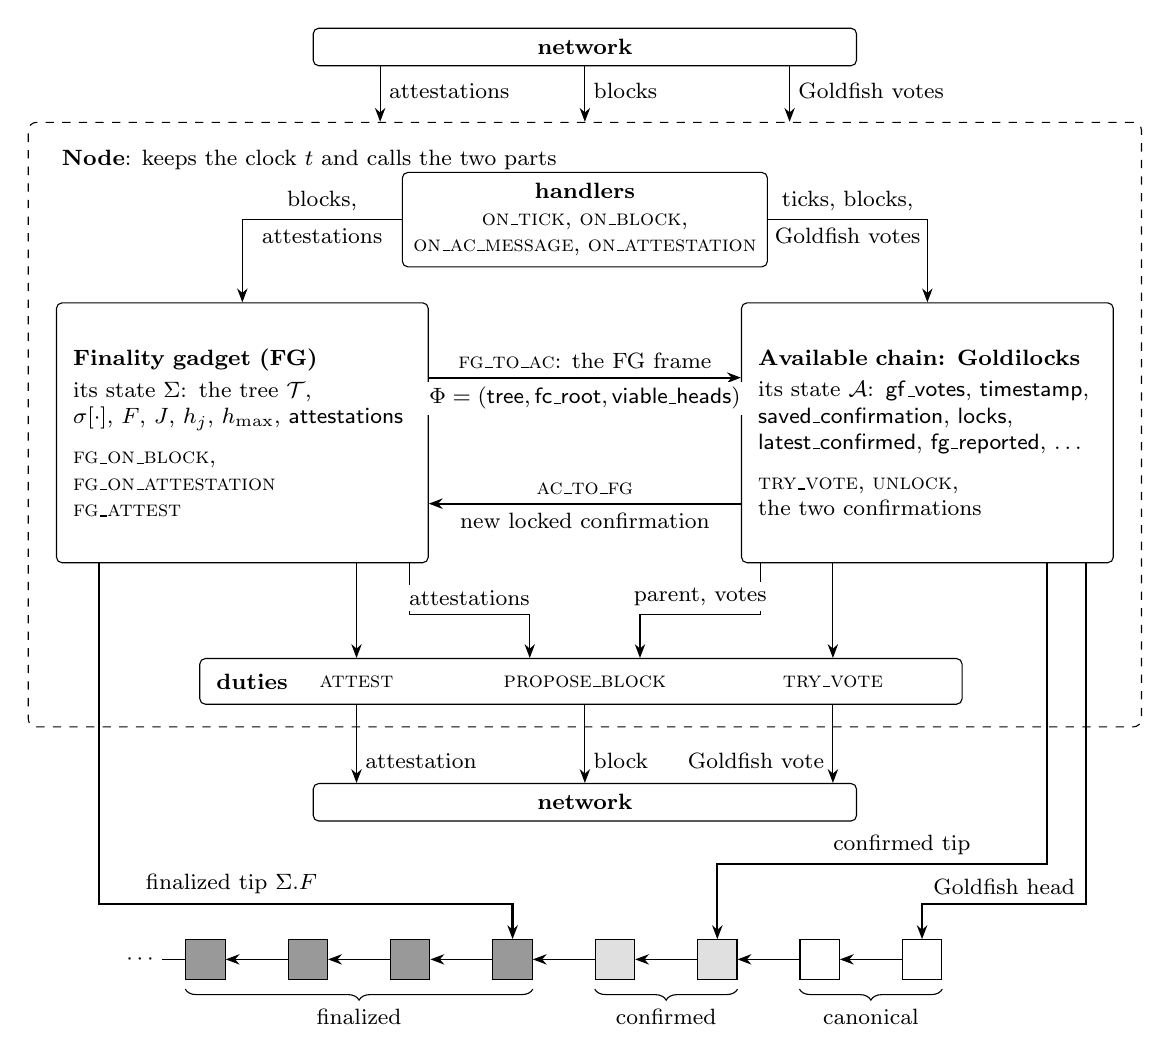
\begin{tikzpicture}[
  font=\footnotesize,
  >={Stealth[length=5pt]},
  part/.style={draw, rounded corners=2pt, align=left, inner sep=6pt,
    text width=4.3cm, minimum height=3.3cm, anchor=north west},
  small/.style={draw, rounded corners=2pt, align=center, inner sep=4pt},
  io/.style={align=center, inner sep=2pt},
  lab/.style={align=center, inner sep=2pt, fill=white},
]
% The two parts.
\node[part] (fg) at (0,0) {%
  \textbf{Finality gadget (FG)}\\[2pt]
  its state~$\Sigma$: the tree~$\T$,\\
  $\sigma[\cdot]$,\ $F$,\ $J$,\ $h_j$,\ $\hmax$, $\attestations$\\[5pt]
  $\fname{fg\_on\_block}$,\ $\fname{fg\_on\_attestation}$\\
  $\fname{fg\_attest}$};
\node[part] (ac) at (8.7,0) {%
  \textbf{Available chain: Goldilocks}\\[2pt]
  its state~$\AC$: $\gfPool$, $\timestamp$,\\
  $\savedConfirmation$, $\locks$,\\
  $\latestConfirmed$, $\fgReported$, \ldots\\[5pt]
  $\fname{try\_vote}$,\ $\fname{unlock}$,\\
  the two confirmations};
% The interface.
\draw[->, thick] ($(fg.east)+(0,0.7)$) -- ($(ac.west)+(0,0.7)$)
  node[lab, midway, above=1pt] {$\fname{fg\_to\_ac}$: the FG frame}
  node[lab, midway, below=1pt] {$\Fr=(\tree,\fcroot,\allowed)$};
\draw[->, thick] ($(ac.west)+(0,-0.9)$) -- ($(fg.east)+(0,-0.9)$)
  node[lab, midway, above=1pt] {$\fname{ac\_to\_fg}$}
  node[lab, midway, below=1pt] {new locked confirmation};
% Handlers.
\node[small] (hand)
  at ($(fg.north east)!0.5!(ac.north west)+(0,1.05)$)
  {\textbf{handlers}\\
   $\fname{on\_tick}$,\ $\fname{on\_block}$,\\
   $\fname{on\_ac\_message}$,\ $\fname{on\_attestation}$};
\draw[->] (hand.west) -| (fg.north)
  node[lab, pos=0.25, above=1pt] {blocks,}
  node[lab, pos=0.25, below=1pt] {attestations};
\draw[->] (hand.east) -| (ac.north)
  node[lab, pos=0.25, above=1pt] {ticks, blocks,}
  node[lab, pos=0.25, below=1pt] {Goldfish votes};
% Duties: one box, narrower than the two parts.
\node[io] (att) at ($(fg.south)+(1.45,-1.5)$) {$\fname{attest}$};
\node[io] (prop) at ($(fg.south east)!0.5!(ac.south west)+(0,-1.5)$)
  {$\fname{propose\_block}$};
\node[io] (vote) at ($(ac.south)+(-1.2,-1.5)$) {$\fname{try\_vote}$};
\node[draw, rounded corners=2pt, inner sep=4pt,
  fit={($(fg.south |- att.north)+(-0.4,0)$)
       ($(ac.south |- att.south)+(0.3,0)$)}] (duties) {};
\node[anchor=west, inner sep=2pt] at ($(duties.west)+(4pt,0)$)
  {\textbf{duties}};
\draw[->] (att.north |- fg.south) -- (att.north |- duties.north);
\draw[->] ($(fg.south east)+(-0.25,0)$) -- ++(0,-0.65)
  -| ($(prop.north |- duties.north)+(-0.7,0)$)
  node[lab, pos=0.25, above=1pt] {attestations};
\draw[->] ($(ac.south west)+(0.25,0)$) -- ++(0,-0.65)
  -| ($(prop.north |- duties.north)+(0.7,0)$)
  node[lab, pos=0.25, above=1pt] {parent, votes};
\draw[->] (vote.north |- ac.south) -- (vote.north |- duties.north);
% The node.
\node[anchor=south west, inner sep=2pt] (title)
  at ($(fg.north west)+(0,1.6)$)
  {\textbf{Node}: keeps the clock~$t$ and calls the two parts};
\node[draw, dashed, rounded corners=3pt, inner xsep=10pt, inner ysep=8pt,
  fit=(fg)(ac)(hand)(title)(duties)] (node) {};
% The network, above and below.
\node[small, minimum width=6.9cm] (netin)
  at ($(hand.north |- node.north)+(0,0.95)$) {\textbf{network}};
\foreach \dx/\txt in {-2.6/attestations, 0/blocks, 2.6/Goldfish votes}
  \draw[->] ($(netin.south)+(\dx,0)$) -- ($(netin.south |- node.north)+(\dx,0)$)
    node[io, pos=0.45, right=1pt] {\txt};
\node[small, minimum width=6.9cm] (netout)
  at ($(prop.south |- node.south)+(0,-0.95)$) {\textbf{network}};
\draw[->] (att.south |- duties.south) -- (att.south |- netout.north)
  node[io, pos=0.72, right=1pt] {attestation};
\draw[->] (prop.south |- duties.south) -- (prop.south |- netout.north)
  node[io, pos=0.72, right=1pt] {block};
\draw[->] (vote.south |- duties.south) -- (vote.south |- netout.north)
  node[io, pos=0.72, left=1pt] {Goldfish vote};
% The chain, with the outputs.
\coordinate (cy) at ($(fg.west |- netout.south)+(0,-1.75)$);
\foreach \i in {0,...,7}
  \node[draw, minimum size=0.5cm, inner sep=0pt] (b\i)
    at ($(cy)+(1.9+1.3*\i,0)$) {};
\foreach \i in {0,...,3}
  \node[draw, fill=black!40, minimum size=0.5cm, inner sep=0pt]
    at (b\i) {};
\foreach \i in {4,5}
  \node[draw, fill=black!12, minimum size=0.5cm, inner sep=0pt]
    at (b\i) {};
\node[io] at ($(b0.west)+(-0.55,0)$) {$\cdots$};
\draw (b0.west) -- ++(-0.3,0);
\foreach \i/\j in {0/1,1/2,2/3,3/4,4/5,5/6,6/7}
  \draw[<-] (b\i.east) -- (b\j.west);
\draw[decorate, decoration={brace, mirror, amplitude=4pt}]
  ($(b0.south west)+(0,-0.12)$) -- ($(b3.south east)+(0,-0.12)$)
  node[io, midway, below=5pt] {finalized};
\draw[decorate, decoration={brace, mirror, amplitude=4pt}]
  ($(b4.south west)+(0,-0.12)$) -- ($(b5.south east)+(0,-0.12)$)
  node[io, midway, below=5pt] {confirmed};
\draw[decorate, decoration={brace, mirror, amplitude=4pt}]
  ($(b6.south west)+(0,-0.12)$) -- ($(b7.south east)+(0,-0.12)$)
  node[io, midway, below=5pt] {canonical};
\draw[->, thick] ($(fg.south west)+(0.55,0)$) |- ($(b3.north)+(0,0.45)$)
  node[io, pos=0.66, above=1pt] {finalized tip $\Sigma.F$}
  -- (b3.north);
\draw[->, thick] ($(ac.south east)+(-0.85,0)$) |- ($(b5.north)+(0,0.95)$)
  node[io, pos=0.72, above=1pt] {confirmed tip}
  -- (b5.north);
\draw[->, thick] ($(ac.south east)+(-0.35,0)$) |- ($(b7.north)+(0,0.45)$)
  node[io, pos=0.75, above=1pt] {Goldfish head}
  -- (b7.north);
\end{tikzpicture}
\caption{Figure~\ref{fig:system} with Goldilocks as the
available chain.  The AC messages are Goldfish votes, the block payload
is the list of previous-slot votes with its support subset, $\mathit{fg\_confirmed}$ is the deepest new viable block at or below a
fast lock of slot $\slot(t)-2$ or later, regular or optimistic, and the
head is the Goldfish head, which the FG does not read.}
\label{fig:goldilocks}
\end{figure}

\subsection{Schedule}\label{sec:sa-schedule}

Slot~$s$ starts at $t_s=4\Delta s$, so $\slot(t)=\lfloor t/(4\Delta)\rfloor$,
and it has the committee $\committee_s=V$.  Slot~$s$ has these public
actions:
\[
\begin{array}{c@{\qquad}l}
 t_s             & \text{proposal, for $s>0$},\\
 \text{at the latest at }t_s+\Delta & \text{Goldfish vote},\\
 \text{before }t_s+2\Delta & \text{optimistic confirmation},\\
 t_s+2\Delta     & \text{confirmation freeze},\\
 t_s+3\Delta     & \text{vote freeze},\\
 \text{before each vote and proposal of slot $s+1$} & \text{unlocking against slot-$s$ votes},\\
 t_s+6\Delta     & \text{confirmation update of slot $s$}.
\end{array}
\]
A node votes in $[t_s,t_s+\Delta]$: as soon as it holds a ready proposal
of slot~$s$, for $s>0$, and else at
$t_s+\Delta$ (Section~\ref{sec:sa-actions}).  Each voter unlocks
immediately before its vote; the proposer also unlocks before its
proposal.  The last two actions of slot~$s$ occur in
slot~$s+1$: the unlocking runs in $[t_{s+1},t_{s+1}+\Delta]$, at the latest
at $t_s+5\Delta=t_{s+1}+\Delta$, and $t_s+6\Delta=t_{s+1}+2\Delta$ is the
confirmation freeze of slot~$s+1$.
Figure~\ref{fig:sa-timeline} shows the two slots.  The formula
$t_s=4\Delta s$ also gives the times of negative~$s$; the pools of a
negative slot are empty.

The parameters are these.
\begin{itemize}
\item $R\geq\lceil(6\Delta+\Delta_F)/(4\Delta)\rceil$ slots per round.  This
  is at least~$2$, because $\Delta_F\geq\Delta$.
\item The slow window of $k\geq2$ slots.  A lock that the confirmation
  update or the optimistic confirmation of slot~$s$ writes is a lock of
  slot~$s$: it lives until $t_{s+k+1}$, the start of slot~$s+k+1$.
\item The FG window $K_W=2$ and the timeout delay
  $\delta_{\mathrm{t}}\geq x+c_F+k_F$ slots (Section~\ref{sec:fg-state}),
  with $c_F=\lceil(6\Delta+\Delta_F)/(4\Delta)\rceil$, the least~$R$, the
  FG slack $k_F\geq0$, and the source delay $x\geq0$ that the finality
  statement below allows.  The default is $x=0$ and
  $\delta_{\mathrm{t}}=c_F+k_F$.  For
  $\Delta_F=\Delta,3\Delta,8\Delta,16\Delta,32\Delta$, $c_F=2,3,4,6,10$;
  $K_W=2$ at every~$\Delta_F$.
\end{itemize}

\emph{Finality liveness (target).}  Take an entry $(h,T_h)$ of slot~$u$
on a chain.  An honest attestation for the entry that is sent by
$t_{u+x}+6\Delta$, the confirmation update of slot~$u+x$, arrives
before $t_{u+x}+6\Delta+\Delta_F\leq t_{u+x+c_F}$, so an honest
node awake from $t_{u+x}+6\Delta$ holds it at the proposal of
slot~$u+x+c_F$ or later.  The \emph{window} of the entry is the slots
$u+x+c_F,\ldots,u+x+c_F+k_F$.  With
$\delta_{\mathrm{t}}\geq x+c_F+k_F$, no block before the last slot of the
window is old enough for the timeout arm, and in a block of that slot the
justification test runs first.  The window is \emph{good} when
\begin{itemize}
\item validators of weight at least~$q$ send a target vote for the entry
  by $t_{u+x}+6\Delta$, or have one on the chain, and at a height whose previous height is justified
  the vote carries the predecessor pair (an honest validator needs to be
  awake and joined, a source with that entry, and a record that allows the
  target and, at such a height, the predecessor pair); and
\item in a slot of the window an honest node, awake from
  $t_{u+x}+6\Delta$, makes a proposal whose parent extends the entry.
\end{itemize}
Then, on the chain of that proposal, at that proposal or before:
\begin{itemize}
\item at a height whose previous height is justified, the height is justified, and its predecessor is
  finalized no later than the justification;
\item at a height whose previous height is not justified, the height is
  justified, and the next height has its previous height justified.
\end{itemize}
A finalization on a chain is the finalized output of a node only when its
finality caches accept it (Section~\ref{sec:fg-frame}).  An honest entry
block gives $x=0$ only when the AC sources the entry at the confirmation
update of slot~$u$: $\fname{ac\_to\_fg}$ can return~$\bot$ or a source
on another chain, so this is an AC obligation, and it is open.  A faulty
entry that honest validators source late has $x>0$; a bound on~$x$ for
faulty entries is open.

A height without a good window can stay current: it crosses by timeout
only in a block at least $\delta_{\mathrm{t}}$ slots after its entry and
with a progress quorum.  At a height whose previous height is justified that crossing appends nothing,
and the predecessor stays pending, but later appends can drop it.  A
later finalization at a height of at least that of the predecessor covers
it: for example, a good window at the next height, whose previous height
is not justified, justifies that height, and a good window at the height
that this justification actually enters, whose previous height is
justified, finalizes it.  A good window at a height whose previous height
is not justified gives its justification, not the finality of the pairs that the
height inherits.

An honest proposal in every $g$ consecutive slots, by a node awake for
the delivery interval and with a parent that extends the entry, gives the
proposal of every window when $k_F\geq g-1$.  It gives neither the rest
of a good window nor good entries: faulty proposers can make every entry.
That good windows recur, once in every $G$ slots for some~$G$, is a
separate target and is open.  For $x=0$ and $k_F=0,1,2,3$ the delay
$\delta_{\mathrm{t}}$ is $c_F,\ldots,c_F+3$: $10$ to $13$ slots at
$\Delta_F=32\Delta$, $3$ to $6$ at $3\Delta$, $2$ to $5$ at~$\Delta$.
These statements are targets.  The window statement and its two-window
form have a paper proof under the premises above; the AC obligations, the
recurrence of good windows, recovery from any state, and every Lean
statement of them are open.

\begin{figure}[!ht]
\centering
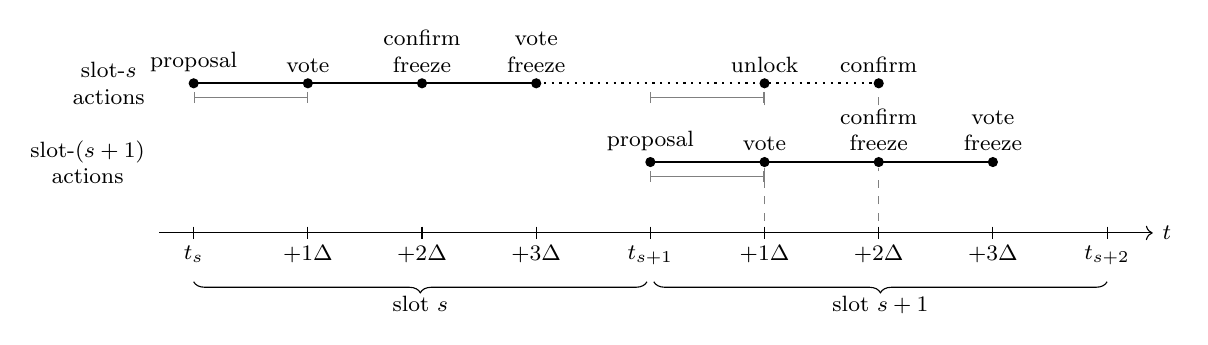
\begin{tikzpicture}[font=\footnotesize, x=1.45cm, y=1cm,
  ev/.style={circle, fill=black, inner sep=1.3pt},
  lab/.style={align=center, inner sep=1pt}]
% Time axis, t_s to t_{s+2}.
\draw[->] (-0.3,0) -- (8.4,0) node[right] {$t$};
\foreach \i in {0,...,8} \draw (\i,0.08) -- (\i,-0.08);
\node[lab, below] at (0,-0.12) {$t_s$};
\foreach \i in {1,2,3} \node[lab, below] at (\i,-0.12) {$+\i\Delta$};
\node[lab, below] at (4,-0.12) {$t_{s+1}$};
\foreach \i/\j in {5/1,6/2,7/3} \node[lab, below] at (\i,-0.12) {$+\j\Delta$};
\node[lab, below] at (8,-0.12) {$t_{s+2}$};
% Slot brackets.
\draw[decorate, decoration={brace, amplitude=4pt, mirror}]
  (0,-0.62) -- (3.97,-0.62) node[lab, midway, below=4pt] {slot $s$};
\draw[decorate, decoration={brace, amplitude=4pt, mirror}]
  (4.03,-0.62) -- (8,-0.62) node[lab, midway, below=4pt] {slot $s+1$};
% Actions of slot s.
\node[lab, anchor=east] at (-0.4,1.9) {slot-$s$\\actions};
\foreach \x/\txt in {0/proposal, 1/vote, 2/{confirm\\freeze}, 3/{vote\\freeze}, 5/unlock, 6/confirm}
  { \node[ev] at (\x,1.9) {}; \node[lab, above] at (\x,2.0) {\txt}; }
\draw[thick] (0,1.9) -- (3,1.9);
\draw[thick, dotted] (3,1.9) -- (6,1.9);
% Actions of slot s+1.
\node[lab, anchor=east] at (-0.4,0.9) {slot-$(s+1)$\\actions};
\foreach \x/\txt in {4/proposal, 5/vote, 6/{confirm\\freeze}, 7/{vote\\freeze}}
  { \node[ev] at (\x,0.9) {}; \node[lab, above] at (\x,1.0) {\txt}; }
\draw[thick] (4,0.9) -- (7,0.9);
% The vote windows: the vote, and the unlocking before it, at the latest at the dot.
\foreach \a/\y in {0/1.72, 4/1.72, 4/0.72}
  \draw[gray, {Bar[width=4pt]}-{Bar[width=4pt]}] (\a,\y) -- (\a+1,\y);
% The two coincidences.
\foreach \x in {5,6} { \draw[dashed, gray] (\x,0.15) -- (\x,0.82);
  \draw[dashed, gray] (\x,1.62) -- (\x,1.82); }
\end{tikzpicture}
\caption{The public actions of slots $s$ and~$s+1$.  A gray bar is a
vote window: a node votes in it, at the latest at its end.  It unlocks
immediately before its vote; the proposer also unlocks before its
proposal.  The confirmation update of slot~$s$ runs in the tick of the
confirmation freeze of slot~$s+1$, before that action
(Section~\ref{sec:sa-actions}).  A node can lock the proposal before the
confirmation freeze (Section~\ref{sec:sa-confirmation}).}
\label{fig:sa-timeline}
\end{figure}

\subsection{State}\label{sec:sa-state}

\[
\begin{split}
 \AC=(&\gfPool[\cdot],\timestamp[\cdot],\savedConfirmation[\cdot],\\
 &\locks,\latestConfirmed,\fgReported,\\
 &\votedSlot,\restartTime).
\end{split}
\]
Table~\ref{tab:sa-state} lists the fields.

\begin{table}[!ht]
\centering
\footnotesize
\begin{tabular}{@{}>{\raggedright\arraybackslash}p{2.9cm}>{\raggedright\arraybackslash}p{3.2cm}>{\raggedright\arraybackslash}p{3.5cm}>{\raggedright\arraybackslash}p{2.7cm}>{\raggedright\arraybackslash}p{1.1cm}@{}}
\hline
Field & Holds & Written by & Read by & Restart\\
\hline
$\gfPool[s]$ & the accepted slot-$s$ votes, at most two distinct votes
  per validator, in the order of acceptance &
  \fname{on\_goldfish\_vote} & vote views, unlocking, confirmation & reset\\
$\timestamp[x]$ & the time at which the AC accepted the vote or block~$x$;
  $\timestamp[\genesis]=-\infty$ &
  \fname{on\_goldfish\_vote}, \fname{ac\_on\_block} &
  resolution, voter block tree & reset\\
$\savedConfirmation[s]$ & the result of the slot-$s$ update, a block
  or~$\bot$, also when a lock vetoes it & \textsc{update\_\allowbreak confirmation} &
  the slow test & reset\\
$\locks$ & the locks $(B,j,f)$: a block, the slot of its confirmation and the fast bit &
  \textsc{update\_\allowbreak confirmation}, \textsc{optimistic\_\allowbreak confirmation}, \textsc{try\_\allowbreak vote}, \fname{ac\_proposal} &
  anchor, veto, unlocking, \fname{ac\_to\_fg} & kept\\
$\latestConfirmed$ & the stored confirmed block, for the confirmed tip &
  \textsc{update\_\allowbreak latest\_\allowbreak confirmed} & \textsc{update\_\allowbreak latest\_\allowbreak confirmed}, \fname{ac\_confirmed} & kept\\
$\fgReported$ & the latest block other than~$\bot$ that the node gave to the FG &
  \fname{ac\_to\_fg} & \fname{ac\_to\_fg} & reset\\
$\votedSlot$ & the slot of the latest vote of the node &
  \textsc{try\_\allowbreak vote} & \textsc{try\_\allowbreak vote} & reset\\
$\restartTime$ & the time of the latest restart & \fname{ac\_restart} &
  \fname{joined} & set\\
\hline
\end{tabular}
\caption{The fields of the Goldilocks state.  The last column says what a
restart does to the field (Section~\ref{sec:sa-joining}).}
\label{tab:sa-state}
\end{table}

The other objects of the rules are derived when they are used, from the
current frame, the AC state and the time tests of their rules: a voter
block tree, a viable tree, a frozen vote set, a score, a set of
opponents, the anchor, and $\mathit{fg\_confirmed}$.

The initial state is $\Call{initial\_ac}{}$ (Figure~\ref{alg:sa-initial}):
empty pools and locks, $\bot$ as the saved confirmation of every integer
slot, also a negative one, and
$\genesis$ as $\AC.\latestConfirmed$ and as $\AC.\fgReported$.

\emph{Joined.}  The node is \emph{joined} at time~$t$ when
$\AC.\restartTime\leq t_{\slot(t)-1}$: it has been awake, with no restart,
since the start of the previous slot.  A node that wakes at $t_j$ is joined
from~$t_{j+1}$, and a node that wakes in $(t_j,t_{j+1})$ is joined
from~$t_{j+2}$.

\captionof{figure}{Goldilocks: initial state and joined}\label{alg:sa-initial}
\nopagebreak
{\footnotesize
\begin{algorithmic}[1]
\Function{initial\_ac}{}
  \State $\AC.\gfPool[s]\gets$ an empty pool, and $\AC.\savedConfirmation[s]\gets\bot$, for every integer $s$
  \State $\AC.\timestamp\gets\{\genesis\mapsto-\infty\}$;\quad $\AC.\locks\gets\emptyset$
  \State $\AC.\latestConfirmed\gets\genesis$;\quad $\AC.\fgReported\gets\genesis$
  \State $\AC.\votedSlot\gets-1$;\quad $\AC.\restartTime\gets-\infty$
  \State \Return $\AC$
\EndFunction
\vspace{1pt}
\Function{joined}{$\AC,t$}
  \State \Return $\AC.\restartTime\leq t_{\slot(t)-1}$
  \Comment{awake since the start of the previous slot}
\EndFunction
\end{algorithmic}
}

\subsection{Votes and views}\label{sec:sa-views}

\emph{The vote.}  The wire message is the Goldfish vote, a tuple
$(\valindex,s,B)$ with $s\geq0$, from validator $\valindex\in\committee_s$
with head~$B$; it names its head by root.  The signer of a slot-$s$ vote
signs it with the slot-$s$ seat of~$\valindex$, under a bijection for each
slot between the seats and $\committee_s=V$.

\emph{The payload.}  The payload of a block is
$B.\acp=(B.\mathsf{votes},B.\mathsf{support\_votes})$: a list of
slot-$(B.\slot-1)$ votes, and a list whose entries occur in
$B.\mathsf{votes}$.  The payload of~$\genesis$ is two empty lists.  With
this payload the digest input of a block is
\[
 (B.\parent.\rootf,\ B.\slot,\ B.\mathsf{attestations},\
 B.\mathsf{votes},\ B.\mathsf{support\_votes}).
\]
The support list records the proposer's view; it is not a second set of
votes to process.  A count reads distinct votes.

\emph{The payload check.}  $\Call{ac\_valid\_payload}{B}$ holds when every
vote in $B.\mathsf{votes}$ has slot $B.\slot-1$ and passes the stateless
checks of a wire vote (its form, its slot, its committee, its signature),
and every entry of $B.\mathsf{support\_votes}$ occurs in
$B.\mathsf{votes}$.  The check reads neither the clock nor the pool.

\emph{Admission.}  $\Call{on\_goldfish\_vote}{}$ accepts a vote at time~$t$
when four conditions hold: its slot is $\slot(t)-1$ or $\slot(t)$, its
validator is in the committee of its slot, the pool does not hold it, and
the pool holds fewer than two distinct votes of its validator for that
slot.  An accepted vote enters the pool with the stamp~$t$.  A vote that
fails a test has no effect.

\emph{Resolution.}  A vote with head~$H$ is \emph{resolved} when
$H\in\Fr.\tree$ and $H.\slot$ is at most the slot of the vote;
$H\in\Fr.\tree$ means that $\Fr.\tree$ holds a block with that root.  The
resolution time of a resolved vote is the later of its stamp and the stamp
of~$H$; the resolution time of any other vote is~$+\infty$.  The test reads
the current FG frame at every use.  A vote whose head is a block of a later
slot than the vote stays in the pool as a cast vote, but it never resolves.

\emph{Vote views.}  A view is a pair of a vote set and its support subset.
$\Call{vote\_view}{}$ takes the slot-$s$ votes held before a cutoff, and as
support the members resolved before it.  $\Call{latest\_view}{}$ takes every
held vote of the latest slot whose votes are due: slot~$s-1$ before
$t_s+2\Delta$, and slot~$s$ from then on.  The head and the proposal read
the latest view.  The vote reads the merged view.

\emph{The merged view.}  The merged view of a slot-$s$ voter is this view:
the slot-$(s-1)$ votes held before the previous-slot vote freeze
$t_{s-1}+3\Delta$, with as support those resolved before it, plus the votes
and the support entries of the slot-$s$ proposals of $\Fr.\tree$, which
pass the freeze.  The support that a proposal declares counts only for
heads in~$\Fr.\tree$ with a slot at most $s-1$.  A proposal outside
$\Fr.\tree$ contributes nothing: the voter cannot vote for it.

\emph{Counting.}  In a set of votes, an \emph{equivocator} is a validator
with two distinct votes.  The \emph{supporters} of a block~$B$ are the
validators that are not equivocators and have a resolved vote in the
support set whose head extends~$B$.

\emph{The voter block tree.}  The block domain of a slot-$s$ voter is the
voter block tree: the blocks of $\Fr.\tree$ received before the
previous-slot vote freeze $t_{s-1}+3\Delta$, and every ancestor of a
current-slot proposal.  The voter takes the viable tree of that tree.  It
does not cut the full viable tree to that tree after the fact: a late
witness cannot make an old pre-freeze child enter the walk of the vote.

\captionof{figure}{Goldilocks: votes and views}\label{alg:sa-views}
\nopagebreak
{\footnotesize
\begin{algorithmic}[1]
\Function{ac\_valid\_payload}{$B$}
  \Comment{stateless: reads neither the clock nor the pool}
  \State \Return $\mathsf{true}$ if every entry of $B.\mathsf{votes}$ is a vote $(v,s,H)$ with $s=B.\slot-1\geq0$, $v\in\committee_s$ and a valid
  \Statex \hspace{2em}signature of the slot-$s$ seat of~$v$, and every entry of $B.\mathsf{support\_votes}$ is in $B.\mathsf{votes}$;
    else $\mathsf{false}$
\EndFunction
\vspace{1pt}
\Function{on\_goldfish\_vote}{$\AC,t,\mathit{vote}$}
  \State $s\gets\slot(t)$
  \If{$\mathit{vote}.\slot<s-1$ or $\mathit{vote}.\slot>s$ or
    $\mathit{vote}.\valindex\notin\committee_{\mathit{vote}.\slot}$ or
    $\mathit{vote}\in\AC.\gfPool[\mathit{vote}.\slot]$}
    \State \Return \EndIf
  \If{$\AC.\gfPool[\mathit{vote}.\slot]$ holds two distinct votes by
    $\mathit{vote}.\valindex$}
    \State \Return \EndIf
  \State add $\mathit{vote}$ to $\AC.\gfPool[\mathit{vote}.\slot]$;
    $\AC.\timestamp[\mathit{vote}]\gets t$
\EndFunction
\vspace{1pt}
\Function{resolution\_time}{$\AC,\Fr,\mathit{vote}$}
  \State $(v,s,H)\gets\mathit{vote}$
  \If{$H\notin\Fr.\tree$ or $H.\slot>s$}
    \State \Return $+\infty$
  \EndIf
  \State \Return $\max\{\AC.\timestamp[\mathit{vote}],\AC.\timestamp[H]\}$
\EndFunction
\vspace{1pt}
\Function{vote\_view}{$\AC,\Fr,s,\mathit{cutoff}$}
  \Comment{the slot-$s$ votes held before the time $\mathit{cutoff}$, and those resolved before it}
  \State $\mathit{votes}\gets\{\mathit{vote}\in\AC.\gfPool[s]:
    \AC.\timestamp[\mathit{vote}]<\mathit{cutoff}\}$, in the order of the pool
  \State $\mathit{support\_votes}\gets\{\mathit{vote}\in\mathit{votes}:
    \Call{resolution\_time}{\AC,\Fr,\mathit{vote}}<\mathit{cutoff}\}$
  \State \Return $(\mathit{votes},\mathit{support\_votes})$
\EndFunction
\vspace{1pt}
\Function{latest\_view}{$\AC,\Fr,t$}
  \State $s\gets\slot(t)$
  \State $s^*\gets s$ if $t\geq t_s+2\Delta$, else $s-1$
    \Comment{the latest slot whose votes are due}
  \State $(\mathit{votes},\mathit{support\_votes})\gets
    \Call{vote\_view}{\AC,\Fr,s^*,+\infty}$
  \Comment{every held vote; the resolved ones}
  \State \Return $(\mathit{votes},\mathit{support\_votes},s^*)$
\EndFunction
\vspace{1pt}
\Function{merged\_vote\_view}{$\AC,\Fr,s$}
  \Comment{the slot-$(s-1)$ view of a slot-$s$ voter}
  \State $\mathit{freeze}\gets t_{s-1}+3\Delta$
  \State $(\mathit{votes},\mathit{support\_votes})\gets
    \Call{vote\_view}{\AC,\Fr,s-1,\mathit{freeze}}$
    \Comment{received, and resolved, before the vote freeze}
  \ForAll{$B\in\Fr.\tree$ with $B.\slot=s$}
    \Comment{the slot-$s$ proposals: their lists pass the vote freeze}
    \State $\mathit{votes}\gets\mathit{votes}\cup B.\mathsf{votes}$
    \State $\mathit{support\_votes}\gets\mathit{support\_votes}\cup
      \{(v,s-1,H)\in B.\mathsf{support\_votes}:H\in\Fr.\tree,\
      H.\slot\leq s-1\}$
  \EndFor
  \State \Return $(\mathit{votes},\mathit{support\_votes})$
\EndFunction
\vspace{1pt}
\Function{equivocators}{$\mathit{votes}$}
  \State \Return $\{v:\mathit{votes}\text{ holds two distinct votes by }v\}$
\EndFunction
\vspace{1pt}
\Function{supporters}{$\mathit{votes},\mathit{support\_votes},s,B$}
  \State \Return $\{v\notin\Call{equivocators}{\mathit{votes}}:
    (v,s,B')\in\mathit{support\_votes}\text{ with }B\preceq B'\}$
\EndFunction
\vspace{1pt}
\Function{voter\_block\_tree}{$\AC,\Fr,s$}
  \State $\mathit{freeze}\gets t_{s-1}+3\Delta$
  \State $\mathit{proposals}\gets\{P\in\Fr.\tree:P.\slot=s\}$
  \State \Return $\{B\in\Fr.\tree:
    \AC.\timestamp[B]<\mathit{freeze}\ \textbf{or}\
    \exists P\in\mathit{proposals},\ B\preceq P\}$
\EndFunction
\vspace{1pt}
\Function{viable\_tree}{$\Fr,\mathit{tree}$}
  \State \Return $\{B\in\mathit{tree}:\Fr.\fcroot\preceq B,\
    \exists W\in\mathit{tree}\cap\Fr.\allowed,\ B\preceq W\}$
\EndFunction
\end{algorithmic}
}

\emph{Fault bound.}  The ``Why'' notes of Section~\ref{sec:sa} write $n$
for the size of the committee, $f$ for the number of faulty validators and
$e\leq f$ for the number of equivocators in a view.  Where a note uses the
fault bound, it is $f<h$, with $h$ the number of joined honest validators.
Then $f<h\leq n-f$, so $2f<n$ and $e<n/2$.  The recovery results use the
stronger bound $f\leq\lfloor(n-1)/3\rfloor$, with their own conditions on
awake nodes and restarts.

\subsection{Locks}\label{sec:sa-locks}

\emph{Locks.}  $\AC.\locks$ is a set of locks $(B,j,f)$: a block, the
slot~$j$ of the confirmation that wrote it, and the fast bit~$f$.  A lock with $f=\mathsf{true}$ is a
\emph{fast lock}: the lock of a fast or an optimistic confirmation
(Section~\ref{sec:sa-confirmation}).  Only $\Call{ac\_to\_fg}{}$ reads the
bit.  A lock is \emph{live} when $\slot(t)\leq j+k$ and $B\in\Fr.\tree$.  This lock
is not the finality lock $\Lambda.\mathsf{lock}[h]$ of the record.

\emph{Lifetimes.}  A \emph{lock of slot~$j$} is a lock with the slot~$j$:
it lives through slot~$j+k$ and is not live from $t_{j+k+1}$ on.  The
optimistic confirmation of slot~$j$ and the confirmation update of
slot~$j$ write the locks of slot~$j$ (Section~\ref{sec:sa-schedule}).  No
later step changes the slot of a lock.  So a lock expires only at the
start of a slot, and no lock expires strictly after~$t_m$ and at or before
$t_m+\Delta$: for fixed stored locks and a fixed frame, every expiry test
gives the same result in the vote window of slot~$m$ and at its proposal.
So expiry alone cannot make an early vote keep a lock that the vote at
$t_m+\Delta$ has lost.  Receipts and lock writes can still change the
effective locks in the window.

\emph{Live locks.}  Every rule reads the locks through
$\Call{live\_locks}{}$, which moves each live lock back to its deepest
ancestor that is in the viable tree or at or below $\Fr.\fcroot$ (at worst
$\Fr.F$), and a block is \emph{locked} when it is at or below the block of
such a lock.

\emph{Why a nonviable lock moves back.}  A lock whose block is viable,
or at or below $\Fr.\fcroot$, keeps its block.  When $\Fr.\fcroot$
advances to a descendant of the block, the root itself protects the
block.  In every other case the FG puts no head on that branch, and the
protection notes of Section~\ref{sec:sa-actions}, which assume that the
block stays in the viable tree of the honest nodes, do not apply to it.
The lock would then only veto the confirmations of the viable branch, and
its moved-back block keeps the protection of the common prefix.

\emph{Effects.}  A live lock has two effects.  Every Goldfish walk of a
duty (Section~\ref{sec:sa-fc}) starts at the \emph{anchor}: the deepest locked block of the full
viable tree $\filtered(\Fr,\Fr.\tree)$, or $\Fr.\fcroot$ when there is no
such block.  $\Call{get\_anchor}{}$ computes it.  A live lock vetoes a confirmation
result~$C$ (Section~\ref{sec:sa-confirmation}) when $C$ conflicts with a
locked block, that is, with the block of a lock of $\Call{live\_locks}{}$;
$\Call{conflicts\_with\_lock}{}$ is this test.

\emph{Adding locks.}  The two confirmations (Section~\ref{sec:sa-confirmation})
add their locks of slot~$s$ through $\Call{add\_locks}{}$.  It returns the
live locks of the stored set and the new locks together, and the caller
stores the result.  So the stored locks are moved back at each write, and
a new lock on a block outside the viable tree is stored on its deepest
ancestor that is viable or at or below $\Fr.\fcroot$: a confirmation
protects only what is viable when it is written.
Without this step, a moved-back lock could become viable again after the
node locked a conflicting block, and two live locks would conflict; with
it, the stored locks lie on one chain.  Each write of $\AC.\latestConfirmed$ comes with such a call,
also an update that adds no lock.  Otherwise a lock that only reads as
moved back could stay stored above its moved-back block while the record
moves to a conflicting branch, and could later read as locked above the
record again.

\emph{Unlocking.}  Unlocking against the slot-$s$ votes runs in
slot~$s+1$, before each vote and each proposal of that slot
(Section~\ref{sec:sa-actions}).  In a view, the \emph{opponents} of a
block~$B'$ are the equivocators of its votes and the validators with a
support vote whose head conflicts with~$B'$.  Unlocking keeps the locks of
slot~$s$ and of later slots.  It moves each other live lock $(B,j,f)$ back
to the deepest~$B'$ with $\Fr.F\preceq B'\preceq B$ for which fewer than
half of the committee are opponents, or to $\Fr.F$ if there is no such
block.  It keeps $j$ and~$f$.  With a fixed frame, evidence slot, view and expiry
tests, unlocking is idempotent.  A lock that is not live changes no
decision; unlocking drops such locks when it runs, and a restart can keep
them.

\emph{Why unlocking is well defined.}  A support vote of a vote view or of
the merged view is resolved (Section~\ref{sec:sa-views}), and the head of
a resolved vote is in $\Fr.\tree$, so the opponents of $\Fr.F$ are only
the equivocators.  These are faulty, so under the fault bound ($e<n/2$)
fewer than half of the committee oppose $\Fr.F$, and the move back stops
at $\Fr.F$ at the latest.  The opponents of an ancestor are a subset of
the opponents of a descendant, so the surviving blocks are a prefix of
$B$'s chain.  A lock on~$\Fr.F$ has no effect.  It does not change the
anchor, because $\Fr.F$ is in the viable tree only when
$\Fr.\fcroot=\Fr.F$, and it vetoes no result
(Section~\ref{sec:sa-confirmation}).  No rule acts on the locks when
$\Fr.F$ advances: a lock whose block left $\Fr.\tree$ is not live, and it
does not become live again, because $\Fr.F$ never moves back.

\emph{The opponents of the merged view.}  At the same frame, every
opponent in the merged view of a slot-$(s+1)$ voter is an opponent in the
whole slot-$s$ pool of the voter.  A carried vote that the pool does not hold was
refused by the two-vote cap, so its validator is an equivocator in the
pool.

\captionof{figure}{Goldilocks: locks and unlocking}\label{alg:sa-locks}
\nopagebreak
{\footnotesize
\begin{algorithmic}[1]
\Function{viable\_ancestor}{$\Fr,B$}
  \Comment{$B\in\Fr.\tree$; $B$ itself when $B$ is viable or below $\Fr.\fcroot$}
  \State \Return the deepest $B'\preceq B$ with $B'\preceq\Fr.\fcroot$ or $B'\in\filtered(\Fr,\Fr.\tree)$
  \Comment{exists: $\Fr.F\preceq\Fr.\fcroot$}
\EndFunction
\vspace{1pt}
\Function{live\_locks}{$\mathit{locks},\Fr,t$}
  \Comment{each moved back: viable, or at or below $\Fr.\fcroot$}
  \State \Return $\{(\Call{viable\_ancestor}{\Fr,B},j,f):(B,j,f)\in\mathit{locks},\ \slot(t)\leq j+k,\ B\in\Fr.\tree\}$
\EndFunction
\vspace{1pt}
\Function{conflicts\_with\_lock}{$\mathit{locks},\Fr,t,C$}
  \Comment{$C$ conflicts with a locked block}
  \State \Return $\mathsf{true}$ if $C$ conflicts with $B_0$ for some $(B_0,j,f)\in\Call{live\_locks}{\mathit{locks},\Fr,t}$, else $\mathsf{false}$
\EndFunction
\vspace{1pt}
\Function{get\_anchor}{$\AC,\Fr,t$}
  \Comment{the deepest viable lock block, or $\Fr.\fcroot$}
  \State $\mathit{blocks}\gets\{B:(B,j,f)\in\Call{live\_locks}{\AC.\locks,\Fr,t}\}$
  \Comment{each viable, or at or below $\Fr.\fcroot$}
  \State \Return the deepest block of $\mathit{blocks}\cup\{\Fr.\fcroot\}$
\EndFunction
\vspace{1pt}
\Function{add\_locks}{$\mathit{locks},\Fr,t,s,N$}
  \Comment{$N$: pairs $(B,f)$, new locks of slot $s$}
  \State \Return $\Call{live\_locks}{\mathit{locks}\cup\{(B,s,f):(B,f)\in N\},\Fr,t}$
  \Comment{the caller writes them}
\EndFunction
\vspace{1pt}
\Function{unlock}{$\mathit{locks},\Fr,t,s,\mathit{votes},\mathit{support\_votes}$}
  \Comment{against the slot-$s$ votes of a view, in slot $s+1$}
  \State $\mathit{equivocators}\gets\Call{equivocators}{\mathit{votes}}$
  \State define $\mathit{opponents}(B')$ as $\mathit{equivocators}\cup\{v:
    (v,s,H)\in\mathit{support\_votes}$
  \Statex \hspace{2em}with $H$ conflicting with $B'\}$
  \State $\mathit{new\_locks}\gets\emptyset$
  \ForAll{$(B,j,f)\in\Call{live\_locks}{\mathit{locks},\Fr,t}$}
    \If{$j<s$}
      \Comment{a lock of slot $s$ or later keeps its place against these votes}
      \State $B\gets$ the deepest $B'\in\Fr.\tree$ with
        $B'\preceq B$ and $2\,|\mathit{opponents}(B')|<|\committee_{s}|$,
        or $\Fr.F$ if there is none
    \EndIf
    \State add $(B,j,f)$ to $\mathit{new\_locks}$
    \Comment{keep the slot and the bit}
  \EndFor
  \State \Return $\mathit{new\_locks}$
  \Comment{the caller writes them}
\EndFunction
\end{algorithmic}
}

\subsection{Fork choice}\label{sec:sa-fc}

\emph{The Goldfish score.}  The Goldfish score of~$B$ is the number of its
supporters plus the number of equivocators: an equivocator counts for
every block.

\emph{The walk.}  A walk starts at a block and descends through the
eligible children: at each step it takes the eligible child with the
greatest score, with ties by root order, and it stops when no child is
eligible.  A child is eligible when its parent is not a viable head, or it
holds a strict majority of the voters, or it is a block of the current
slot.  A walk starts at its start block also when that block is not in the
tree that it walks.

\emph{The head.}  $\Call{ac\_head}{}$ computes the head when it is read: a
walk of the full viable tree with the latest view.  It reads the current
frame and the current locks, so a change of~$\Fr$ moves it at once.
At~$t_s$ it is the head of the proposal, and in a pair for the FG it is the head of
the pair.  The vote duty reads a frozen voter block tree, so its
head can differ.

\emph{Why the head waits for no honest vote.}  An honest node votes at the
latest at $t_s+\Delta$.  When the delivery bounds hold from~$t_s$ and the
node is awake from $t_s+\Delta$, every honest vote of slot~$s$ reaches it
before $t_s+2\Delta$, the time from which the head reads slot~$s$.

\captionof{figure}{Goldilocks: fork choice}\label{alg:sa-fc}
\nopagebreak
{\footnotesize
\begin{algorithmic}[1]
\Function{goldfish\_score}{$\mathit{votes},\mathit{support\_votes},s,B$}
  \State \Return $|\Call{equivocators}{\mathit{votes}}|+
    |\Call{supporters}{\mathit{votes},\mathit{support\_votes},s,B}|$
  \Comment{equivocators count for every block}
\EndFunction
\vspace{1pt}
\Function{goldfish\_eligible}{$\Fr,t,\mathit{votes},
  \mathit{support\_votes},s,B$}
  \If{$B.\parent\notin\Fr.\allowed$} \State \Return $\mathsf{true}$
    \Comment{the walk is not yet on a viable head}
  \EndIf
  \If{$B.\slot=\slot(t)$} \State \Return $\mathsf{true}$
    \Comment{a block of the current slot}
  \EndIf
  \State $\mathit{voters\_count}\gets
    |\{v:\mathit{votes}\text{ holds a vote by }v\}|$
  \State $\mathit{score}\gets\Call{goldfish\_score}{\mathit{votes},
    \mathit{support\_votes},s,B}$
  \State \Return $2\,\mathit{score}>\mathit{voters\_count}$
  \Comment{a strict majority of the voters}
\EndFunction
\vspace{1pt}
\Function{ghost}{$\mathit{anchor},\mathit{tree},
  \mathit{score},\mathit{eligible}$}
  \State $H\gets\mathit{anchor}$
  \Loop
    \State $\mathit{children}\gets\{B:B\text{ is a child of }H\text{ in }
      \mathit{tree},\ \mathit{eligible}(B)\}$
    \If{$\mathit{children}=\emptyset$} \State \Return $H$ \EndIf
    \State $H\gets\arg\max_{B\in\mathit{children}}\mathit{score}(B)$,
      ties by root order
  \EndLoop
\EndFunction
\vspace{1pt}
\Function{get\_head}{$\AC,\Fr,t,\mathit{tree},
  \mathit{votes},\mathit{support\_votes},s$}
  \State $\mathit{anchor}\gets\Call{get\_anchor}{\AC,\Fr,t}$
  \Comment{of the full viable tree, also when $\mathit{tree}$ is smaller}
  \State define $\mathit{score}(B)$ as
  \Statex \hspace{2em}
    $\Call{goldfish\_score}{\mathit{votes},\mathit{support\_votes},s,B}$
  \State define $\mathit{eligible}(B)$ as
  \Statex \hspace{2em}
    $\Call{goldfish\_eligible}{\Fr,t,\mathit{votes},
      \mathit{support\_votes},s,B}$
  \State \Return $\Call{ghost}{\mathit{anchor},\mathit{tree},
    \mathit{score},\mathit{eligible}}$
\EndFunction
\vspace{1pt}
\Function{ac\_head}{$\AC,\Fr,t$}
  \State $(\mathit{votes},\mathit{support\_votes},s^*)\gets
    \Call{latest\_view}{\AC,\Fr,t}$
  \State \Return $\Call{get\_head}{\AC,\Fr,t,\filtered(\Fr,\Fr.\tree),
    \mathit{votes},\mathit{support\_votes},s^*}$
  \Comment{the head of the full viable tree}
\EndFunction
\end{algorithmic}
}

\subsection{Confirmation}\label{sec:sa-confirmation}

At $t_s+6\Delta$ the AC evaluates slot~$s$ once.  The update runs in the
tick at $t_s+6\Delta$, before the objects of that time, so every vote and
block that it reads has an earlier stamp.

\emph{The latest confirmed block.}
$\Call{update\_latest\_confirmed}{}$ writes $\AC.\latestConfirmed$ for
the two confirmation rules: an ancestor of the stored block leaves it
unchanged, and an extension or a conflicting block replaces it.  No voting
rule reads it.

\emph{The result.}  The result of the update is the deepest block of
$\Fr.\tree$ at or above~$\Fr.F$ that holds a strict majority of the
participants of the slot, and $\bot$ when there is none.  Support counts
only the votes resolved before $t_s+2\Delta$, the confirmation freeze, of
validators with no second vote, and the participants are the validators
with a vote.  Such a validator supports one branch only, so two
conflicting blocks cannot both hold the majority, and an ancestor has at
least the support of its descendant: the blocks that hold it lie on one
chain.

\emph{The saved result and the veto.}  The update saves the result in
$\AC.\savedConfirmation[s]$, also when a live lock vetoes it, for the slow
test of later slots.  A live lock that conflicts with the result vetoes it
(Section~\ref{sec:sa-locks}).  A lock on~$\Fr.F$ vetoes no result, because
every result extends~$\Fr.F$.  An update with no result or with a vetoed
result changes neither $\AC.\latestConfirmed$ nor the locks.  Otherwise
the update updates $\AC.\latestConfirmed$ with the result.

\emph{The locks.}  Then the update writes locks of slot~$s$
(Section~\ref{sec:sa-locks}) on non-genesis blocks of the result's chain
in $\Fr.\tree$, by two tests.  The fast test: half of the committee or
more supports the block.  The slow test: the saved confirmations of the
previous $k-1$ slots are all in $\Fr.\tree$ and extend the block.  The
update writes a fast lock on the deepest block~$D$ that passes the fast
test, if there is one, and a lock that is not fast on the deepest block
that passes the slow test, when there is no~$D$ or that block is deeper
than~$D$.  An ancestor has at least
the support of its descendant, so the blocks of the chain up to~$D$ pass
the fast test, and a fast lock on~$D$ covers them.  As every new lock, these
locks are stored moved back (Section~\ref{sec:sa-locks}), so a stored
block can be a strict ancestor of the selected block, also~$\genesis$.

\emph{The fast locks for the FG.}  A live fast lock of slot~$j$ is a
source for the FG in the slots $j$, $j+1$ and~$j+2$
(Section~\ref{sec:sa-actions}).  It stays a lock while it is live, but the
move back of $\Call{live\_locks}{}$ or an unlocking can move its block
back before that time, and the source moves back with it.  The window is two slots because the
update of slot~$j$ writes in slot~$j+1$: its fast lock stays a source
through the optimistic confirmations of slot~$j+2$, so an optimistic
confirmation of an ancestor does not take the place of a deeper fast
lock.  A failed confirmation writes no lock, so it removes no source.  A
lock that is not fast is never a source.  The record
$\AC.\latestConfirmed$ serves the user.

\emph{The optimistic confirmation.}  In a slot $s>0$, before
$t_s+2\Delta$, a joined node checks after each receipt
(Section~\ref{sec:sa-actions}) the blocks~$B$ of $\Fr.\tree$.  A
block~$B$ passes when at least three quarters of the committee have a
slot-$s$ vote in its pool whose head extends~$B$, equivocators included,
and $B$ conflicts with no locked block.  For the deepest passing block,
the node adds a fast lock of slot~$s$, stored moved back as every new
lock, and updates $\AC.\latestConfirmed$.
Its lock is the lock of a fast confirmation; only the trigger differs.  If two conflicting blocks passed,
at least half of the committee would have votes that extend each of them;
under the fault bound ($e<n/2$) the passing blocks thus lie on one chain.
A block of slot~$s$ passes when the votes for it pass; an older block, for
example the parent of a late proposal, can pass with votes for several of
its descendants.  A later receipt in the slot can make a deeper block
pass.  An optimistic confirmation does not change the saved result, and
the update of slot~$s$ still runs at $t_s+6\Delta$.

\emph{The confirmed tip.}  $\Call{ac\_confirmed}{}$ takes
$\AC.\latestConfirmed$ when it is in $\Fr.\tree$, and $\Fr.F$ otherwise, and returns the deepest common
ancestor of that block and the head of $\Call{ac\_head}{}$.  So the
confirmed tip is never ahead of the head, and it can step back while the
head is behind $\AC.\latestConfirmed$ or on another branch.

\captionof{figure}{Goldilocks: confirmation}\label{alg:sa-gate}
\nopagebreak
{\footnotesize
\begin{algorithmic}[1]
\Function{update\_latest\_confirmed}{$\AC,\Fr,C$}
  \Comment{$C$ is confirmed}
  \State $E\gets\AC.\latestConfirmed$
  \If{$E\notin\Fr.\tree$ or $C\not\preceq E$}
    \State $\AC.\latestConfirmed\gets C$
    \Comment{never back to an ancestor}
  \EndIf
\EndFunction
\vspace{1pt}
\Function{confirmation\_score}{$\AC,\Fr,s,B$}
  \State $\mathit{votes}\gets\AC.\gfPool[s]$
  \Comment{the whole pool: it decides who equivocates}
  \State $\mathit{early}\gets\{\mathit{vote}\in\mathit{votes}:
    \Call{resolution\_time}{\AC,\Fr,\mathit{vote}}<t_s+2\Delta\}$
  \State \Return $|\Call{supporters}{\mathit{votes},\mathit{early},s,B}|$
  \Comment{early, non-equivocating support}
\EndFunction
\vspace{1pt}
\Function{get\_confirmation}{$\AC,\Fr,s$}
  \Comment{at $t_s+6\Delta$; every stamp is below it}
  \State $\mathit{voters\_count}\gets
    |\{v:\AC.\gfPool[s]\text{ holds a vote by }v\}|$
  \State \Return the deepest $B\in\Fr.\tree$ with $\Fr.F\preceq B$ and
    $2\,\Call{confirmation\_score}{\AC,\Fr,s,B}>\mathit{voters\_count}$,
  \Statex \hspace{2em}or $\bot$ if there is none
  \Comment{a strict majority of the voters; these blocks lie on one chain}
\EndFunction
\vspace{1pt}
\Function{update\_confirmation}{$\AC,\Fr,t,s$}
  \Comment{at $t_s+6\Delta$}
  \State $C\gets\Call{get\_confirmation}{\AC,\Fr,s}$
  \State $\AC.\savedConfirmation[s]\gets C$
  \If{$C\neq\bot$ and not \Call{conflicts\_with\_lock}{$\AC.\locks,\Fr,t,C$}}
    \Comment{else no result, or a vetoed one}
    \State \Call{update\_latest\_confirmed}{$\AC,\Fr,C$}
    \State $\mathit{path}\gets\{B\in\Fr.\tree:B\neq\genesis,\ B\preceq C\}$
    \State define $\mathit{fast}(B)$ as
      $2\,\Call{confirmation\_score}{\AC,\Fr,s,B}\geq|\committee_s|$
    \Comment{the fast test}
    \State define $\mathit{slow}(B)$ as: every $j$ with $s-k<j<s$ has
      $\AC.\savedConfirmation[j]\in\Fr.\tree$
    \Statex \hspace{5.5em}and $B\preceq\AC.\savedConfirmation[j]$
    \Comment{the slow test}
    \State $D\gets$ the deepest $B\in\mathit{path}$ with $\mathit{fast}(B)$, or $\bot$ if there is none
    \State $\mathit{lock\_block}\gets$ the deepest $B\in\mathit{path}$ with
      $\mathit{fast}(B)$ or $\mathit{slow}(B)$, or $\bot$ if there is none
    \State $N\gets\{(D,\mathsf{true})\}$ if $D\neq\bot$, else $\emptyset$
    \Comment{the fast lock}
    \If{$\mathit{lock\_block}\neq D$}
      \Comment{a slow block, deeper than $D$ or with no $D$}
      \State $N\gets N\cup\{(\mathit{lock\_block},\mathsf{false})\}$
    \EndIf
    \State $\AC.\locks\gets\Call{add\_locks}{\AC.\locks,\Fr,t,s,N}$
    \Comment{also when $N=\emptyset$}
  \EndIf
\EndFunction
\vspace{1pt}
\Function{optimistic\_confirmation}{$\AC,\Fr,t$}
  \Comment{after each receipt}
  \State $s\gets\slot(t)$
  \If{not \Call{joined}{$\AC,t$} or $s=0$ or $t\geq t_s+2\Delta$}
    \State \Return
  \EndIf
  \State define $\mathit{voters}(B)$ as
    $\{v:(v,s,H)\in\AC.\gfPool[s]\text{ with }H\in\Fr.\tree\text{ and }B\preceq H\}$
  \Comment{equivocators included}
  \State define $\mathit{passes}(B)$ as $4\,|\mathit{voters}(B)|\geq3\,|\committee_s|$
  \Statex \hspace{4em}and not \Call{conflicts\_with\_lock}{$\AC.\locks,\Fr,t,B$}
  \State $B\gets$ a deepest $B\in\Fr.\tree$ with $\mathit{passes}(B)$, or $\bot$ if there is none
  \Comment{if $e<n/2$, they lie on one chain}
  \If{$B=\bot$}
    \State \Return
  \EndIf
  \State $\AC.\locks\gets\Call{add\_locks}{\AC.\locks,\Fr,t,s,\{(B,\mathsf{true})\}}$
  \State \Call{update\_latest\_confirmed}{$\AC,\Fr,B$}
\EndFunction
\vspace{1pt}
\Function{ac\_confirmed}{$\AC,\Fr,t$}
  \Comment{user-facing; no protocol rule reads it}
  \State $C\gets\AC.\latestConfirmed$ if $\AC.\latestConfirmed\in\Fr.\tree$,
    else $\Fr.F$
  \State $H\gets\Call{ac\_head}{\AC,\Fr,t}$
  \State \Return the deepest common ancestor of $C$ and $H$
  \Comment{never ahead of the head}
\EndFunction
\end{algorithmic}
}

\subsection{Node actions}\label{sec:sa-actions}

This section gives the event handlers and the duties of the AC.

\emph{The joined test.}  Only a joined node (Section~\ref{sec:sa-state})
unlocks, votes, confirms optimistically, proposes, runs the confirmation
update or gives a block to the FG.  A node that is not joined still
computes a head from the votes that it holds: $\Call{ac\_head}{}$ has no
such test.

\emph{When the node votes.}  For $s>0$, a joined node casts its slot-$s$
vote at the first time $\tau\in[t_s,t_s+\Delta]$ at which it holds a \emph{ready} proposal: a block $P\in\Fr.\tree$
with $P.\slot=s$ whose support references are resolved, that is, every
$(v,s-1,H)$ in $P.\mathsf{support\_votes}$ has $H\in\Fr.\tree$ and
$H.\slot\leq s-1$.  If no such time comes before
$t_s+\Delta$, the node votes at $t_s+\Delta$ with no test, as it does in
slot~$0$.  The vote check $\Call{try\_vote}{}$ runs after each receipt and
in the tick at $t_s+\Delta$, and it tests that the node is joined at~$\tau$.
The vote is one sequence: the unlocking against the slot-$(s-1)$ votes
(Section~\ref{sec:sa-locks}); then the vote; then the own vote enters
through $\Call{ac\_on\_message}{}$, which runs the optimistic check.  In
the same sequence, $\AC.\votedSlot$ records the slot of the vote, so a
node votes once per slot, and the unlocking before its vote runs once per
slot.

\emph{The vote.}  At its vote time~$\tau$ the voter walks a frozen view,
and it reads the frame, the locks and the proposals at~$\tau$.  It walks
the viable tree of its voter block tree with its merged view
(Section~\ref{sec:sa-views}), and the unlocking before the vote reads the
same merged view.  The vote is the head of that walk.

\emph{The checks after a receipt.}  After each block and each vote, the
handlers first check for an optimistic confirmation
(Section~\ref{sec:sa-confirmation}) and then run the vote check
$\Call{try\_vote}{}$, so they take the
frame.  So a receipt handler can send the vote of the node, as the tick
can.  The node processes its own vote as a receipt, so the optimistic
check also follows its own vote.

\captionof{figure}{Goldilocks: the vote and the vote receipt}\label{alg:sa-vote}
\nopagebreak
{\footnotesize
\begin{algorithmic}[1]
\Function{vote\_ready}{$\Fr,s$}
  \Comment{a ready proposal of slot $s$}
  \State \Return $\exists P\in\Fr.\tree$ with $P.\slot=s$ such that every
    $(v,s-1,H)\in P.\mathsf{support\_votes}$
  \Statex \hspace{2em}has $H\in\Fr.\tree$ and $H.\slot\leq s-1$
\EndFunction
\vspace{1pt}
\Function{try\_vote}{$\AC,\Fr,t$}
  \Comment{after each receipt, and in the tick at $t_s+\Delta$}
  \State $s\gets\slot(t)$
  \If{not \Call{joined}{$\AC,t$} or $\AC.\votedSlot=s$ or $t>t_s+\Delta$}
    \State \Return
    \Comment{one vote per slot}
  \EndIf
  \If{$t<t_s+\Delta$ and ($s=0$ or not \Call{vote\_ready}{$\Fr,s$})}
    \State \Return
    \Comment{wait for a ready proposal or for $t_s+\Delta$}
  \EndIf
  \State $(\mathit{votes},\mathit{support\_votes})\gets
    \Call{merged\_vote\_view}{\AC,\Fr,s}$
  \Comment{the view of the vote; empty in slot 0}
  \If{$s>0$}
    \State $\AC.\locks\gets\Call{unlock}{\AC.\locks,\Fr,t,s-1,\mathit{votes},\mathit{support\_votes}}$
  \EndIf
  \State $\mathit{tree}\gets
    \filtered(\Fr,\Call{voter\_block\_tree}{\AC,\Fr,s})$
  \State $H\gets\Call{get\_head}{\AC,\Fr,t,\mathit{tree},
    \mathit{votes},\mathit{support\_votes},s-1}$
  \State $\AC.\votedSlot\gets s$
  \Comment{before the own vote, which re-enters this check}
  \If{$\valindex\in\committee_s$}
    \State $\mathit{vote}\gets(\valindex,s,H)$; broadcast $\mathit{vote}$;
      \Call{ac\_on\_message}{$\AC,\Fr,t,\mathit{vote}$}
    \Comment{the own vote is a receipt}
  \EndIf
\EndFunction
\vspace{1pt}
\Function{ac\_on\_message}{$\AC,\Fr,t,\mathit{vote}$}
  \State \Call{on\_goldfish\_vote}{$\AC,t,\mathit{vote}$}
  \State \Call{optimistic\_confirmation}{$\AC,\Fr,t$}
  \State \Call{try\_vote}{$\AC,\Fr,t$}
  \Comment{can send the vote of the node}
\EndFunction
\end{algorithmic}
}

\emph{Why a marker for the one vote.}  A test for the own vote in the pool
would also be sound: only the validator signs its votes, and admission
accepts its first vote of the current slot.  The marker does not depend on
admission, and the vote sequence writes it.  A restart resets it, but a
node that restarts in slot~$s$ is not joined in slot~$s$, so it does not
vote again in that slot.

\emph{Blocks.}  When the FG accepts a block~$B$, the node calls
$\Call{ac\_on\_block}{}$.  It stamps $B$ with the clock and gives each vote
of $B.\mathsf{votes}$ to the admission test.

\emph{The tick.}  The tick of a node that is not joined does nothing
(Section~\ref{sec:sa-state}).  For a joined node, at $t_s+\Delta$ the tick
runs the vote check.  If the node has not voted in slot~$s$, the check
first unlocks against the slot-$(s-1)$ votes, for $s>0$, and then casts
the vote of slot~$s$.  At
$t_s+2\Delta$, for $s>0$, the tick runs the confirmation update of
slot~$s-1$.  A tick runs before the objects of its time
(Section~\ref{sec:node}), so the vote check and the update of the tick
read only objects with an earlier stamp.  The
proposal at~$t_s$ and the FG update are duties of the node; they run after
the tick and call $\Call{ac\_proposal}{}$ and $\Call{ac\_to\_fg}{}$.
Before it proposes, $\Call{ac\_proposal}{}$ unlocks against the
slot-$(s-1)$ votes.

\emph{The proposal.}  At~$t_s$, for $s>0$, the proposer puts every
previous-slot vote that it holds in $B.\mathsf{votes}$, in the order of its
pool, and exactly the members resolved at proposal time in
$B.\mathsf{support\_votes}$, in the same order.  Its parent is the head of
$\Call{ac\_head}{}$ after the unlocking against its whole slot-$(s-1)$
pool, with the resolved votes as support (Section~\ref{sec:sa-locks}).
At slot~$0$ the head is genesis.  The proposer processes its own block at
once, so it can vote at~$t_s$; it unlocks again before that vote, with
the frame and the view of the vote.  The second call need not leave the
locks unchanged: the own block can advance~$\Fr.F$ or change the viable
tree.  So unlocking against the slot-$s$ votes runs in
$[t_{s+1},t_{s+1}+\Delta]$, at the latest at $t_s+5\Delta$.

\emph{The block for the FG.}  After each tick, a joined node gives the FG
a new block when it has one.  The candidates are the blocks of the live
fast locks of slot $\slot(t)-2$ or later that are in the full viable
tree.  A live lock block outside the viable tree is at or below
$\Fr.\fcroot$, and so are its ancestors, so no viable block below it is
lost.  The locked blocks lie on one chain, because a lock
write is vetoed by a conflicting lock and unlocking only moves a lock
back, so the candidates lie on one chain and the head extends them.  The node gives the block when the deepest candidate exists and is
not an ancestor of $\AC.\fgReported$, the block that it gave last, or
equal to it.  A block given earlier that left $\Fr.\tree$ has no
candidate as an ancestor.  So at each tick of a joined node the FG gets
the deepest candidate when it is new, which covers the chain up to it, and
a block on another branch when the confirmations move there.

\captionof{figure}{Goldilocks: block, tick, proposal and FG update}\label{alg:sa-events}
\nopagebreak
{\footnotesize
\begin{algorithmic}[1]
\Function{ac\_on\_block}{$\AC,\Fr,t,B$}
  \State $\AC.\timestamp[B]\gets t$
  \ForAll{$\mathit{vote}\in B.\mathsf{votes}$}
    \State \Call{on\_goldfish\_vote}{$\AC,t,\mathit{vote}$}
  \EndFor
  \State \Call{optimistic\_confirmation}{$\AC,\Fr,t$}
  \State \Call{try\_vote}{$\AC,\Fr,t$}
  \Comment{can send the vote of the node}
\EndFunction
\vspace{1pt}
\Function{ac\_on\_tick}{$\AC,\Fr,t$}
  \State $s\gets\slot(t)$
  \If{not \Call{joined}{$\AC,t$}} \State \Return
    \Comment{not joined: no duty and no write}
  \EndIf
  \If{$t=t_s+\Delta$}
    \State \Call{try\_vote}{$\AC,\Fr,t$}
    \Comment{the latest vote time: no readiness test}
  \EndIf
  \If{$t=t_s+2\Delta$ and $s>0$}
    \State \Call{update\_confirmation}{$\AC,\Fr,t,s-1$}
  \EndIf
\EndFunction
\vspace{1pt}
\Function{ac\_proposal}{$\AC,\Fr,t$}
  \Comment{runs at $t_s$: the view is of slot $s-1$}
  \If{not \Call{joined}{$\AC,t$}} \State \Return $\bot$
    \Comment{not joined: the node makes no proposal}
  \EndIf
  \State $s\gets\slot(t)$
  \State $(\mathit{votes},\mathit{support\_votes})\gets
    \Call{vote\_view}{\AC,\Fr,s-1,+\infty}$
  \Comment{every previous-slot vote held; the resolved ones}
  \State $\AC.\locks\gets\Call{unlock}{\AC.\locks,\Fr,t,s-1,\mathit{votes},\mathit{support\_votes}}$
  \State $H\gets\Call{get\_head}{\AC,\Fr,t,\filtered(\Fr,\Fr.\tree),
    \mathit{votes},\mathit{support\_votes},s-1}$
  \Comment{the head of $\Call{ac\_head}{}$}
  \State \Return $(H,(\mathit{votes},\mathit{support\_votes}))$
\EndFunction
\vspace{1pt}
\Function{ac\_to\_fg}{$\AC,\Fr,t$}
  \Comment{after each tick}
  \If{not \Call{joined}{$\AC,t$}} \State \Return $\bot$ \EndIf
  \State $\mathit{cands}\gets\{B:(B,j,\mathsf{true})\in\Call{live\_locks}{\AC.\locks,\Fr,t},\ \slot(t)\leq j+2,\ B\in\filtered(\Fr,\Fr.\tree)\}$
  \If{$\mathit{cands}=\emptyset$} \State \Return $\bot$ \EndIf
  \State $C\gets$ the deepest block of $\mathit{cands}$
  \Comment{the candidates lie on one chain}
  \If{$\AC.\fgReported\in\Fr.\tree$ and $C\preceq\AC.\fgReported$} \State \Return $\bot$
    \Comment{nothing new}
  \EndIf
  \State $\AC.\fgReported\gets C$
  \State \Return $C$
\EndFunction
\end{algorithmic}
}

\emph{Why the vote can be early.}  The vote freeze $t_{s-1}+3\Delta=t_s-\Delta$
comes before~$t_s$, so in the vote window no receipt changes the part of
the view that the freeze bounds.  An early vote differs from a vote at
$t_s+\Delta$ in the slot-$s$ proposals that it merges, in the frame, and
in the locks that later receipts write, for example an optimistic
confirmation of slot~$s$.  A ready proposal contributes all of its declared support, because
every support entry resolves.

\emph{Why locks expire at slot starts.}  Expiry alone cannot make an
early vote keep a lock that the vote at $t_s+\Delta$ has lost
(Section~\ref{sec:sa-locks}).  A lock of slot~$s$ is live at no proposal and no vote of
slot~$s+k+1$; the slow first transfer reads the votes of that slot
without the lock.  The cost: with the previous deadline $t_{s+k}+5\Delta$ the
proposal and the early votes of slot~$s+k+1$ also read the lock, so a lock
now lives $(4k-2)\Delta$ after its write at $t_s+6\Delta$, not
$(4k-1)\Delta$, and the outage budget is $\Delta$ smaller.

\emph{Latency.}  Suppose an honest proposer sends~$P$ at~$t_s$, an actual
delay $\delta<\Delta$ from~$t_s$ on, and at least three quarters of the
committee honest, awake and joined.  Suppose each of them holds a ready~$P$
by $t_s+\delta$, and its vote rule selects~$P$.  Then their votes reach an
awake node by $t_s+2\delta<t_s+2\Delta$.  If that node is joined, holds~$P$
and has no conflicting locked block, it confirms~$P$ optimistically by
then.  This remark is conditional; it is not a bound that this section
proves.

\emph{Why equivocators are opponents.}  An optimistic confirmation counts votes
before the equivocations are known (Section~\ref{sec:sa-confirmation}).
Take another honest node that is joined in slot~$s+1$, does not restart
in between, and accepts the heads of the counted votes and their
ancestors in time, and these heads stay in $\Fr.\tree$ until its
unlocking.  The counted votes and their heads reach it before the vote
freeze $t_s+3\Delta$, so under the delivery bounds the votes are resolved
in the view of its unlocking.  In
that view, each validator
that the first node counted is either a voter whose head extends its
block, so an opponent of every block that conflicts with it, or an
equivocator.  So that node releases every lock
that conflicts with the lock of the optimistic confirmation, except a lock
of slot~$s$ or~$s+1$, which keeps its place against the slot-$s$ votes;
the note ``Why an optimistic
confirmation is a fast confirmation'' below
shows when no such lock can conflict.  The bound on the opponents of a protected lock does not
change: honest validators never equivocate, so every equivocator is
faulty, and the opponents are at most the honest opponents and the faulty
validators, as before.

\emph{Why a lock of slot~$s$ keeps its place.}  The slot-$s$ votes are the
evidence of a lock of slot~$s$.  As opponents, the equivocators among them
could move the lock back.  The regular locks of slot~$s$ do not meet this
unlocking either: the update writes them at $t_s+6\Delta$, after the
unlocking, which runs at the latest at $t_s+5\Delta$.  The later
unlockings apply to them as to every lock.  A lock of slot~$s+1$ can also
exist at this unlocking.  The other honest nodes can vote early, so a
node can hold three quarters of the committee as slot-$(s+1)$ voters for
a block, and confirm it optimistically, before its own vote of
slot~$s+1$ and thus before this unlocking.  The slot-$s$ votes are not the
evidence of that lock, and the rule keeps it in its place.  The first
unlocking that can move it against opponents is the one against the
slot-$(s+2)$ votes, as for the regular locks of slot~$s+1$.  The move back
of $\Call{live\_locks}{}$ applies to every lock, also to these.

\emph{Why the proposer and the voters agree on the unlocking.}  Suppose
synchrony, an honest proposer of slot~$s+1$ and the same frame.  Then the
view of the proposal and the merged view of each voter that holds the
proposal give the same opponents for each block.  A vote that the voter
received before the vote freeze $t_s+3\Delta$ reaches the proposer
before $t_{s+1}$.  The proposal carries every slot-$s$ vote of the
proposer, with the resolved ones as support.  The raw vote sets can
differ because of the two-vote cap, but a vote that the cap refuses at
the proposer makes its validator an equivocator at both nodes.  So the
proposal and the votes agree on the unlocking; nodes with different
locks before it can still hold different locks after it.  A second
unlocking over a larger view could move a lock further back, so each node
unlocks once for its vote; the proposer also unlocks before its proposal.

\emph{Why the view keeps the bounds on protected locks.}  At the same
frame, every opponent in the merged view of a slot-$(s+1)$ voter is an
opponent in its whole slot-$s$ pool (Section~\ref{sec:sa-locks}).  So each bound on the opponents of a
protected lock holds as with the whole pool.  The release arguments use
only votes and blocks that arrive before the vote freeze, and these are in
the view.

\emph{Why an optimistic confirmation is a fast confirmation.}  Write $n=|\committee_s|$ and
let $S$ be the validators that the node counted.  The node received their
votes and the heads of these votes before $t_s+2\Delta$, and it forwards
them.  Take an honest node that is joined in slot~$s+1$, does not restart
in between, and accepts these heads and their ancestors in time.  It
holds, before the vote freeze $t_s+3\Delta$, for each member of~$S$ either
the resolved counted vote, whose head extends~$B$, or two other votes of
that validator, which make it an equivocator.  Before
its vote of slot~$s+1$, it unlocks against the slot-$s$ votes of its view,
and this view holds every vote received before the vote freeze
(Section~\ref{sec:sa-locks}).  The earliest such unlocking is at
$t_{s+1}=t_s+4\Delta$, after the vote freeze, so the time of the unlocking
in $[t_{s+1},t_{s+1}+\Delta]$ does not change the argument.  Each member
of~$S$ is an opponent of every lock that conflicts with~$B$
(Section~\ref{sec:sa-locks}), and $|S|\geq 3n/4$, so every such lock moves
back, except a lock of slot~$s+1$.  Suppose that every honest node that votes
in slot~$s+1$ is such a node, and that $B$ stays in its viable voter block
tree at that vote.  Take the honest votes of slot~$s+1$ in the order of
their events.  A lock of slot~$s+1$ that conflicts with~$B$
needs an optimistic confirmation of slot~$s+1$, so three quarters of the
committee with votes that extend a block that conflicts with~$B$.  At most $f<n/2$
of them are faulty, so at least one of them is an honest vote that
conflicts with~$B$.  At the first such honest vote, its node has no lock
of slot~$s+1$ that conflicts with~$B$.  It has no conflicting lock of
slot~$s$ either: two optimistic confirmations of slot~$s$ cannot conflict,
and the update of slot~$s$ runs after the vote window.  So all its
conflicting locks moved back.  Then its walk
then compares the child toward~$B$, with a Goldfish score of at
least~$|S|$, with any conflicting child, whose score is at most
$e+n-|S|<|S|$, where $e<n/2$ is the number of equivocators, and the vote
extends~$B$, a contradiction.  So every such vote extends~$B$, as after a
fast lock.  Suppose that at least half of the
committee are such nodes, and that a node holds their slot-$(s+1)$ votes,
resolved, before $t_{s+1}+2\Delta$.  Then the result of slot~$s+1$ at that node
extends~$B$, because $2h>h+f$ for the $h$ honest voters, and, if
$B\neq\genesis$, its fast test locks $B$ or a descendant of~$B$.  Genesis
needs no lock: every block extends it.  As for a fast lock, the protection of~$B$ at the other
nodes thus starts at the update of slot~$s+1$, at $t_{s+1}+6\Delta$, under
the same participation, delivery and frame conditions: an optimistic confirmation shows~$B$ earlier,
but it does not protect~$B$ earlier against an outage.  Two conflicting blocks cannot both pass: they would
need half of the committee as common voters, all of them equivocators.

\emph{Why the FG can take every confirmation.}  The FG needs a block that
the next honest votes extend.  A fast confirmation and an optimistic
confirmation give this under the same conditions
(Section~\ref{sec:sa-confirmation} and the note ``Why an optimistic
confirmation is a fast confirmation'' above), and the protection of an optimistic
confirmation against an outage starts at the same time as that of the
fast confirmation of its slot.  Only fast locks are sources, and an
unlocking that moves a fast lock back moves the source back.  A fast lock
of slot~$j$ is a source while it is live and $\slot(t)\leq j+2$.  Its
block is viable, or at or below $\Fr.\fcroot$, when the lock is written,
but the FG can still get it
later than its confirmation: the block can leave the viable tree and come
back before the next lock write.  That the next honest votes then still
extend the block has a paper proof, not yet in Lean, for both origins.
The first transfer uses the evidence of the confirmation, and each later
slot uses the honest votes of the slot before it, so no new lock is
needed, also after the source lock expires.  The proof needs synchrony
from slot~$j$ on, delivery and acceptance of the counted votes and of
each later honest batch with their heads, no restart that erases them,
in each slot honest votes of at least half of the committee (to release
a conflicting old lock), and the block on the viable voting path of each
voter.  The local lock and viability at the call do not prove it.  From slot $\slot(\tau)+3$ on, every source is a fast lock
written after the time~$\tau$, so the sources of the healing argument can
be counted from the fast locks written after GST.  The client record of the FG gives at most
one target per height, so more pairs do not give more targets per height:
they let a validator vote as soon as its chain enters a new height.  This
note covers the age of the sources and the safety of the client.  That the finality
bounds stay as before with these earlier attestations is a proof
obligation: the present proofs assume one honest FG action per round.

\subsection{Joining and restart}\label{sec:sa-joining}

\emph{Restart.}  A restart keeps the locks and $\AC.\latestConfirmed$, and it resets
every other part of~$\AC$ to its initial value.  It sets
$\AC.\restartTime$ to the time of the restart, and it calls
$\Call{ac\_on\_block}{}$ at that time for every block of $\Fr.\tree$ other
than~$\genesis$, in parent order.  Any order in which every block comes after
its parent is correct: the replay at a restart in slot~$s'$ admits only votes
of slots below~$s'$, and a node joined at~$t$ has $s'\leq\slot(t)-1$ and reads
only votes of slot $\slot(t)-1$ or later, so the order of siblings changes no
pool or stamp that a joined node reads.  These blocks get that stamp, and the
votes that they carry and that admission accepts enter the pools with it.
A lock written before a restart keeps its slot, so a sleep does not
extend it.  The restart resets $\AC.\votedSlot$.
A node that restarts in slot~$s$ is not joined in slot~$s$, so it does not
unlock or vote a second time in that slot.  The replay of the blocks runs
the optimistic check and the vote check of $\Call{ac\_on\_block}{}$, but
the node is not joined at the time of the restart, so both checks do
nothing.

\emph{Before the node joins.}  A node that is not joined has run no
update since its restart.  So its saved confirmations stay~$\bot$, as the
restart left them.  The locks stay, fast locks included: after the node
joins, a fast lock written before the restart is a source for the FG
while its window lasts.

\emph{Why the node must join.}  A restart erases the votes that the node
received before it, faulty early votes included, and the network need not
deliver them again.  An action after such a restart could read a different
set of votes than the other honest nodes.  A node does not accept a
slot-$j$ vote before~$t_j$, and a block carries slot-$j$ votes only from
slot~$j+1$.  So a node joined at~$t$ has erased no vote of slot
$\slot(t)-1$ or later, and every action of the tick reads only such votes:
the vote, the proposal and unlocking read slot~$s-1$ in
$[t_s,t_s+\Delta]$, the optimistic confirmation reads slot~$s$, and the
update of slot~$s-1$ runs at $t_s+2\Delta$.  When the
delivery bounds hold from $t_{s-1}$, a joined node also holds every
honest slot-$(s-1)$ vote before $t_{s-1}+2\Delta$, so before the vote freeze
$t_{s-1}+3\Delta$.  It also receives every block and AC message sent while
it slept before $t_{s-1}+2\Delta$.  Receipt is not acceptance: the node
keeps such an object only if it passes admission.  For example, it refuses
a delayed vote of a slot below $\slot(t)-1$.  (Attestations have the
bound~$\Delta_F$, and the AC does not read them.)

\captionof{figure}{Goldilocks: restart}\label{alg:sa-restart}
\nopagebreak
{\footnotesize
\begin{algorithmic}[1]
\Function{ac\_restart}{$\AC,\Fr,t$}
  \Comment{the node restarts at $t$}
  \State $\AC'\gets\Call{initial\_ac}{}$
  \State $\AC'.\locks\gets\AC.\locks$;\quad
    $\AC'.\latestConfirmed\gets\AC.\latestConfirmed$
  \Comment{they persist}
  \State $\AC'.\restartTime\gets t$
  \ForAll{$B\in\Fr.\tree$ with $B\neq\genesis$, in parent order}
    \State \Call{ac\_on\_block}{$\AC',\Fr,t,B$}
    \Comment{stamps the block and its votes with $t$}
  \EndFor
  \State \Return $\AC'$
\EndFunction
\end{algorithmic}
}

\end{document}
